% Options for packages loaded elsewhere
\PassOptionsToPackage{unicode}{hyperref}
\PassOptionsToPackage{hyphens}{url}
\PassOptionsToPackage{dvipsnames,svgnames,x11names}{xcolor}
%
\documentclass[
  letterpaper,
  DIV=11,
  numbers=noendperiod]{scrartcl}

\usepackage{amsmath,amssymb}
\usepackage{iftex}
\ifPDFTeX
  \usepackage[T1]{fontenc}
  \usepackage[utf8]{inputenc}
  \usepackage{textcomp} % provide euro and other symbols
\else % if luatex or xetex
  \usepackage{unicode-math}
  \defaultfontfeatures{Scale=MatchLowercase}
  \defaultfontfeatures[\rmfamily]{Ligatures=TeX,Scale=1}
\fi
\usepackage{lmodern}
\ifPDFTeX\else  
    % xetex/luatex font selection
\fi
% Use upquote if available, for straight quotes in verbatim environments
\IfFileExists{upquote.sty}{\usepackage{upquote}}{}
\IfFileExists{microtype.sty}{% use microtype if available
  \usepackage[]{microtype}
  \UseMicrotypeSet[protrusion]{basicmath} % disable protrusion for tt fonts
}{}
\makeatletter
\@ifundefined{KOMAClassName}{% if non-KOMA class
  \IfFileExists{parskip.sty}{%
    \usepackage{parskip}
  }{% else
    \setlength{\parindent}{0pt}
    \setlength{\parskip}{6pt plus 2pt minus 1pt}}
}{% if KOMA class
  \KOMAoptions{parskip=half}}
\makeatother
\usepackage{xcolor}
\setlength{\emergencystretch}{3em} % prevent overfull lines
\setcounter{secnumdepth}{5}
% Make \paragraph and \subparagraph free-standing
\ifx\paragraph\undefined\else
  \let\oldparagraph\paragraph
  \renewcommand{\paragraph}[1]{\oldparagraph{#1}\mbox{}}
\fi
\ifx\subparagraph\undefined\else
  \let\oldsubparagraph\subparagraph
  \renewcommand{\subparagraph}[1]{\oldsubparagraph{#1}\mbox{}}
\fi

\usepackage{color}
\usepackage{fancyvrb}
\newcommand{\VerbBar}{|}
\newcommand{\VERB}{\Verb[commandchars=\\\{\}]}
\DefineVerbatimEnvironment{Highlighting}{Verbatim}{commandchars=\\\{\}}
% Add ',fontsize=\small' for more characters per line
\usepackage{framed}
\definecolor{shadecolor}{RGB}{241,243,245}
\newenvironment{Shaded}{\begin{snugshade}}{\end{snugshade}}
\newcommand{\AlertTok}[1]{\textcolor[rgb]{0.68,0.00,0.00}{#1}}
\newcommand{\AnnotationTok}[1]{\textcolor[rgb]{0.37,0.37,0.37}{#1}}
\newcommand{\AttributeTok}[1]{\textcolor[rgb]{0.40,0.45,0.13}{#1}}
\newcommand{\BaseNTok}[1]{\textcolor[rgb]{0.68,0.00,0.00}{#1}}
\newcommand{\BuiltInTok}[1]{\textcolor[rgb]{0.00,0.23,0.31}{#1}}
\newcommand{\CharTok}[1]{\textcolor[rgb]{0.13,0.47,0.30}{#1}}
\newcommand{\CommentTok}[1]{\textcolor[rgb]{0.37,0.37,0.37}{#1}}
\newcommand{\CommentVarTok}[1]{\textcolor[rgb]{0.37,0.37,0.37}{\textit{#1}}}
\newcommand{\ConstantTok}[1]{\textcolor[rgb]{0.56,0.35,0.01}{#1}}
\newcommand{\ControlFlowTok}[1]{\textcolor[rgb]{0.00,0.23,0.31}{#1}}
\newcommand{\DataTypeTok}[1]{\textcolor[rgb]{0.68,0.00,0.00}{#1}}
\newcommand{\DecValTok}[1]{\textcolor[rgb]{0.68,0.00,0.00}{#1}}
\newcommand{\DocumentationTok}[1]{\textcolor[rgb]{0.37,0.37,0.37}{\textit{#1}}}
\newcommand{\ErrorTok}[1]{\textcolor[rgb]{0.68,0.00,0.00}{#1}}
\newcommand{\ExtensionTok}[1]{\textcolor[rgb]{0.00,0.23,0.31}{#1}}
\newcommand{\FloatTok}[1]{\textcolor[rgb]{0.68,0.00,0.00}{#1}}
\newcommand{\FunctionTok}[1]{\textcolor[rgb]{0.28,0.35,0.67}{#1}}
\newcommand{\ImportTok}[1]{\textcolor[rgb]{0.00,0.46,0.62}{#1}}
\newcommand{\InformationTok}[1]{\textcolor[rgb]{0.37,0.37,0.37}{#1}}
\newcommand{\KeywordTok}[1]{\textcolor[rgb]{0.00,0.23,0.31}{#1}}
\newcommand{\NormalTok}[1]{\textcolor[rgb]{0.00,0.23,0.31}{#1}}
\newcommand{\OperatorTok}[1]{\textcolor[rgb]{0.37,0.37,0.37}{#1}}
\newcommand{\OtherTok}[1]{\textcolor[rgb]{0.00,0.23,0.31}{#1}}
\newcommand{\PreprocessorTok}[1]{\textcolor[rgb]{0.68,0.00,0.00}{#1}}
\newcommand{\RegionMarkerTok}[1]{\textcolor[rgb]{0.00,0.23,0.31}{#1}}
\newcommand{\SpecialCharTok}[1]{\textcolor[rgb]{0.37,0.37,0.37}{#1}}
\newcommand{\SpecialStringTok}[1]{\textcolor[rgb]{0.13,0.47,0.30}{#1}}
\newcommand{\StringTok}[1]{\textcolor[rgb]{0.13,0.47,0.30}{#1}}
\newcommand{\VariableTok}[1]{\textcolor[rgb]{0.07,0.07,0.07}{#1}}
\newcommand{\VerbatimStringTok}[1]{\textcolor[rgb]{0.13,0.47,0.30}{#1}}
\newcommand{\WarningTok}[1]{\textcolor[rgb]{0.37,0.37,0.37}{\textit{#1}}}

\providecommand{\tightlist}{%
  \setlength{\itemsep}{0pt}\setlength{\parskip}{0pt}}\usepackage{longtable,booktabs,array}
\usepackage{calc} % for calculating minipage widths
% Correct order of tables after \paragraph or \subparagraph
\usepackage{etoolbox}
\makeatletter
\patchcmd\longtable{\par}{\if@noskipsec\mbox{}\fi\par}{}{}
\makeatother
% Allow footnotes in longtable head/foot
\IfFileExists{footnotehyper.sty}{\usepackage{footnotehyper}}{\usepackage{footnote}}
\makesavenoteenv{longtable}
\usepackage{graphicx}
\makeatletter
\def\maxwidth{\ifdim\Gin@nat@width>\linewidth\linewidth\else\Gin@nat@width\fi}
\def\maxheight{\ifdim\Gin@nat@height>\textheight\textheight\else\Gin@nat@height\fi}
\makeatother
% Scale images if necessary, so that they will not overflow the page
% margins by default, and it is still possible to overwrite the defaults
% using explicit options in \includegraphics[width, height, ...]{}
\setkeys{Gin}{width=\maxwidth,height=\maxheight,keepaspectratio}
% Set default figure placement to htbp
\makeatletter
\def\fps@figure{htbp}
\makeatother

% load packages
\usepackage{geometry}
\usepackage{xcolor}
\usepackage{eso-pic}
\usepackage{fancyhdr}
\usepackage{sectsty}
\usepackage{fontspec}
\usepackage{titlesec}

%% Set page size with a wider right margin
\geometry{a4paper, total={170mm,257mm}, left=20mm, top=20mm, bottom=20mm, right=50mm}

%% Let's define some colours
\definecolor{uniblue}{HTML}{003865}
\definecolor{burgundy}{HTML}{7D2239}
\definecolor{cobalt}{HTML}{005C8A}
\definecolor{lavender}{HTML}{5B4D94}
\definecolor{leaf}{HTML}{006630}
\definecolor{moss}{HTML}{385A4F}
\definecolor{pillarbox}{HTML}{B30C00}
\definecolor{rust}{HTML}{9A3A06}
\definecolor{sandstone}{HTML}{52473B}
\definecolor{skyblue}{HTML}{005398}
\definecolor{slate}{HTML}{4F5961}
\definecolor{thistle}{HTML}{951272}

%\definecolor{light}{HTML}{E6E6FA} % original from template - redefined below as uni blue at 10 percent:
\colorlet{light}{uniblue!10}
%\definecolor{highlight}{HTML}{800080} % original from template - redefined below as uni's skyblue:
\colorlet{highlight}{skyblue}
%\definecolor{dark}{HTML}{330033} % original from template - redefined below as uni blue at 100 percent:
\colorlet{dark}{uniblue}

%% Let's add the border on the right hand side 
\AddToShipoutPicture{% 
    \AtPageLowerLeft{% 
        \put(\LenToUnit{\dimexpr\paperwidth-3cm},0){% 
            \color{light}\rule{3cm}{\LenToUnit\paperheight}%
          }%
     }%
     % logo
    \AtPageLowerLeft{% start the bar at the bottom right of the page
        \put(\LenToUnit{\dimexpr\paperwidth-2.25cm},27.2cm){% move it to the top right
            \color{light}
\includegraphics[width=2.25cm]{_extensions/nrennie/PrettyPDF/uni_logo_boxed.jpg}
          }%
     }%
}

%% Style the page number
\fancypagestyle{mystyle}{
  \fancyhf{}
  \renewcommand\headrulewidth{0pt}
  \fancyfoot[R]{\thepage}
  \fancyfootoffset{3.5cm}
}
\setlength{\footskip}{20pt}

%% style the chapter/section fonts
\chapterfont{\color{uniblue}\fontsize{20}{16.8}\selectfont}
\sectionfont{\color{uniblue}\fontsize{20}{16.8}\selectfont}
\subsectionfont{\color{skyblue}\fontsize{14}{16.8}\selectfont}
\titleformat{\subsection}
  {\color{uniblue!90}\sffamily\Large\bfseries}{\thesubsection}{1em}{}[{\titlerule[0.8pt]}]
\subsubsectionfont{\color{cobalt}}

\renewcommand\thesection{\color{slate}\arabic{section}}
  
% left align title
\makeatletter
\renewcommand{\maketitle}{\bgroup\setlength{\parindent}{0pt}
\begin{flushleft}
  {\color{uniblue}\sffamily\huge\textbf{\@title}} \vspace{0.3cm} \newline
  {\Large {\@subtitle}} \newline
  \@author
\end{flushleft}\egroup
}
\makeatother

%% Use some custom fonts
\setsansfont{Ubuntu}[
    Path=_extensions/nrennie/PrettyPDF/Ubuntu/,
    Scale=0.9,
    Extension = .ttf,
    UprightFont=*-Regular,
    BoldFont=*-Bold,
    ItalicFont=*-Italic,
    ]

\setmainfont{Ubuntu}[
    Path=_extensions/nrennie/PrettyPDF/Ubuntu/,
    Scale=0.9,
    Extension = .ttf,
    UprightFont=*-Regular,
    BoldFont=*-Bold,
    ItalicFont=*-Italic,
    ]
\usepackage{booktabs}
\usepackage{longtable}
\usepackage{array}
\usepackage{multirow}
\usepackage{wrapfig}
\usepackage{float}
\usepackage{colortbl}
\usepackage{pdflscape}
\usepackage{tabu}
\usepackage{threeparttable}
\usepackage{threeparttablex}
\usepackage[normalem]{ulem}
\usepackage{makecell}
\usepackage{xcolor}
\KOMAoption{captions}{tableheading}
\makeatletter
\@ifpackageloaded{tcolorbox}{}{\usepackage[skins,breakable]{tcolorbox}}
\@ifpackageloaded{fontawesome5}{}{\usepackage{fontawesome5}}
\definecolor{quarto-callout-color}{HTML}{909090}
\definecolor{quarto-callout-note-color}{HTML}{0758E5}
\definecolor{quarto-callout-important-color}{HTML}{CC1914}
\definecolor{quarto-callout-warning-color}{HTML}{EB9113}
\definecolor{quarto-callout-tip-color}{HTML}{00A047}
\definecolor{quarto-callout-caution-color}{HTML}{FC5300}
\definecolor{quarto-callout-color-frame}{HTML}{acacac}
\definecolor{quarto-callout-note-color-frame}{HTML}{4582ec}
\definecolor{quarto-callout-important-color-frame}{HTML}{d9534f}
\definecolor{quarto-callout-warning-color-frame}{HTML}{f0ad4e}
\definecolor{quarto-callout-tip-color-frame}{HTML}{02b875}
\definecolor{quarto-callout-caution-color-frame}{HTML}{fd7e14}
\makeatother
\makeatletter
\@ifpackageloaded{caption}{}{\usepackage{caption}}
\AtBeginDocument{%
\ifdefined\contentsname
  \renewcommand*\contentsname{Table of contents}
\else
  \newcommand\contentsname{Table of contents}
\fi
\ifdefined\listfigurename
  \renewcommand*\listfigurename{List of Figures}
\else
  \newcommand\listfigurename{List of Figures}
\fi
\ifdefined\listtablename
  \renewcommand*\listtablename{List of Tables}
\else
  \newcommand\listtablename{List of Tables}
\fi
\ifdefined\figurename
  \renewcommand*\figurename{Figure}
\else
  \newcommand\figurename{Figure}
\fi
\ifdefined\tablename
  \renewcommand*\tablename{Table}
\else
  \newcommand\tablename{Table}
\fi
}
\@ifpackageloaded{float}{}{\usepackage{float}}
\floatstyle{ruled}
\@ifundefined{c@chapter}{\newfloat{codelisting}{h}{lop}}{\newfloat{codelisting}{h}{lop}[chapter]}
\floatname{codelisting}{Listing}
\newcommand*\listoflistings{\listof{codelisting}{List of Listings}}
\makeatother
\makeatletter
\makeatother
\makeatletter
\@ifpackageloaded{caption}{}{\usepackage{caption}}
\@ifpackageloaded{subcaption}{}{\usepackage{subcaption}}
\makeatother
\makeatletter
\@ifpackageloaded{tcolorbox}{}{\usepackage[skins,breakable]{tcolorbox}}
\makeatother
\makeatletter
\@ifundefined{shadecolor}{\definecolor{shadecolor}{rgb}{.97, .97, .97}}{}
\makeatother
\makeatletter
\@ifundefined{codebgcolor}{\definecolor{codebgcolor}{named}{light}}{}
\makeatother
\makeatletter
\ifdefined\Shaded\renewenvironment{Shaded}{\begin{tcolorbox}[frame hidden, sharp corners, colback={codebgcolor}, boxrule=0pt, enhanced, breakable]}{\end{tcolorbox}}\fi
\makeatother
\ifLuaTeX
  \usepackage{selnolig}  % disable illegal ligatures
\fi
\usepackage{bookmark}

\IfFileExists{xurl.sty}{\usepackage{xurl}}{} % add URL line breaks if available
\urlstyle{same} % disable monospaced font for URLs
\hypersetup{
  pdftitle={Week 1: Visualising and data tidying using R},
  colorlinks=true,
  linkcolor={highlight},
  filecolor={Maroon},
  citecolor={Blue},
  urlcolor={highlight},
  pdfcreator={LaTeX via pandoc}}

\title{Week 1: Visualising and data tidying using R}
\author{}
\date{}

\begin{document}
\maketitle

\pagestyle{mystyle}

\section{Getting started}\label{getting-started}

This week we will review various techniques for data \textbf{tidying},
\textbf{wrangling} and \textbf{visualization} in R. We'll revisit key
concepts from your previous \textbf{R programming} course and build on
them with more advanced methods for data manipulation and plotting.

\begin{tcolorbox}[enhanced jigsaw, title=\textcolor{quarto-callout-note-color}{\faInfo}\hspace{0.5em}{Note}, bottomtitle=1mm, leftrule=.75mm, toprule=.15mm, opacityback=0, arc=.35mm, colbacktitle=quarto-callout-note-color!10!white, bottomrule=.15mm, colback=white, coltitle=black, titlerule=0mm, toptitle=1mm, colframe=quarto-callout-note-color-frame, opacitybacktitle=0.6, rightrule=.15mm, left=2mm, breakable]

A lot of the content within this course is based on the open-source book
\href{https://moderndive.com/index.html}{Statistical Inference via Data
Science} and thus is a useful source for additional examples and
questions.

\end{tcolorbox}

First, start by opening \textbf{RStudio} by going to
\texttt{Desktop\ -\textgreater{}\ Maths-Stats\ -\textgreater{}\ RStudio}.
Once RStudio has opened create a new R script by going to
\texttt{File\ -\textgreater{}\ New\ File\ -\textgreater{}\ R\ Script}.
Next go to \texttt{File\ -\textgreater{}\ Save\ As...} and save the
script into your personal drive. Alternatively, you can download today's
session R script and open it on RStudio (remember to save any edits or
comments you make on this file) :

We shall now load into R all of the libraries we will need for this
session. This can be done by typing the following into your R script:

\begin{Shaded}
\begin{Highlighting}[]
\FunctionTok{library}\NormalTok{(ggplot2)}
\FunctionTok{library}\NormalTok{(tidyverse)}
\FunctionTok{library}\NormalTok{(nycflights13)}
\FunctionTok{library}\NormalTok{(fivethirtyeight)}
\end{Highlighting}
\end{Shaded}

The libraries can be loaded into R by highlighting them in your script
and then clicking on the \texttt{Run} button located in the top right of
the script window. The first library \texttt{ggplot2} allows us to use
functions within that package in order to create nice data
visualisations. The \texttt{tidyverse} library is actually a collection
of different R packages for manipulating data. The final two libraries
(\texttt{nycflights13} and \texttt{fivethirtyeight}) contain interesting
data sets that we shall examine in this session.

Notice that when loading the \texttt{tidyverse} package you get a
message that tells you about conflicting functions of certain packages.
This means that there is at least one or more functions with the same
name loaded from different packages (and thus one the function will mask
the other).

\begin{enumerate}
\def\labelenumi{\arabic{enumi}.}
\item
  Using \texttt{::} after calling the package name every time we use the
  function from that package. E.g., \texttt{dplyr::filter(…)} will tell
  R to explicitly use the function \texttt{filter} from the
  \texttt{dplyr} library.
\item
  Load the \texttt{conflicted} library and use the
  \texttt{conflicts\_prefer("function","package")} function to
  explicitly declare which version of the function you want to use in
  the remaining R session (i.e.~after \texttt{conflicts\_prefer()} is
  called, e.g., \texttt{conflict\_prefer("filter","dplyr")} .
\end{enumerate}

\begin{tcolorbox}[enhanced jigsaw, title={Question}, bottomtitle=1mm, leftrule=.75mm, toprule=.15mm, opacityback=0, arc=.35mm, colbacktitle=quarto-callout-tip-color!10!white, bottomrule=.15mm, colback=white, coltitle=black, titlerule=0mm, toptitle=1mm, colframe=quarto-callout-tip-color-frame, opacitybacktitle=0.6, rightrule=.15mm, left=2mm, breakable]

What do you think is the advantage of using the
\texttt{conflicts\_prefer} as opposed to the first approach?

\end{tcolorbox}

\section{Viewing the data}\label{viewing-the-data}

Before visualising any data set, we first need to know its contents. For
example, the contents of the \texttt{flights} data within the
\texttt{nycflights13} library can be observed using the following
command:

\begin{Shaded}
\begin{Highlighting}[]
\FunctionTok{glimpse}\NormalTok{(flights)}
\end{Highlighting}
\end{Shaded}

\begin{verbatim}
Rows: 336,776
Columns: 19
$ year           <int> 2013, 2013, 2013, 2013, 2013, 2013, 2013, 2013, 2013, 2~
$ month          <int> 1, 1, 1, 1, 1, 1, 1, 1, 1, 1, 1, 1, 1, 1, 1, 1, 1, 1, 1~
$ day            <int> 1, 1, 1, 1, 1, 1, 1, 1, 1, 1, 1, 1, 1, 1, 1, 1, 1, 1, 1~
$ dep_time       <int> 517, 533, 542, 544, 554, 554, 555, 557, 557, 558, 558, ~
$ sched_dep_time <int> 515, 529, 540, 545, 600, 558, 600, 600, 600, 600, 600, ~
$ dep_delay      <dbl> 2, 4, 2, -1, -6, -4, -5, -3, -3, -2, -2, -2, -2, -2, -1~
$ arr_time       <int> 830, 850, 923, 1004, 812, 740, 913, 709, 838, 753, 849,~
$ sched_arr_time <int> 819, 830, 850, 1022, 837, 728, 854, 723, 846, 745, 851,~
$ arr_delay      <dbl> 11, 20, 33, -18, -25, 12, 19, -14, -8, 8, -2, -3, 7, -1~
$ carrier        <chr> "UA", "UA", "AA", "B6", "DL", "UA", "B6", "EV", "B6", "~
$ flight         <int> 1545, 1714, 1141, 725, 461, 1696, 507, 5708, 79, 301, 4~
$ tailnum        <chr> "N14228", "N24211", "N619AA", "N804JB", "N668DN", "N394~
$ origin         <chr> "EWR", "LGA", "JFK", "JFK", "LGA", "EWR", "EWR", "LGA",~
$ dest           <chr> "IAH", "IAH", "MIA", "BQN", "ATL", "ORD", "FLL", "IAD",~
$ air_time       <dbl> 227, 227, 160, 183, 116, 150, 158, 53, 140, 138, 149, 1~
$ distance       <dbl> 1400, 1416, 1089, 1576, 762, 719, 1065, 229, 944, 733, ~
$ hour           <dbl> 5, 5, 5, 5, 6, 5, 6, 6, 6, 6, 6, 6, 6, 6, 6, 5, 6, 6, 6~
$ minute         <dbl> 15, 29, 40, 45, 0, 58, 0, 0, 0, 0, 0, 0, 0, 0, 0, 59, 0~
$ time_hour      <dttm> 2013-01-01 05:00:00, 2013-01-01 05:00:00, 2013-01-01 0~
\end{verbatim}

This function provides a concise overview of a data frame's structure.
For each column/variable, it displays the name, data type, and a brief
preview of the actual values along with dimensions of the data set (i.e,
19 columns and 336776 rows).

Another useful function that can be used to quickly explore your data is
the \texttt{slice()} function. It allows you to extract specific rows
from a data frame based on their positions.

For example, \texttt{slice(flights,\ 1:5)} retrieves the first 5 rows of
the \texttt{flights} data frame. Additionally, the \texttt{.by} argument
in \texttt{slice()} enables grouped slicing
(e.g.~\texttt{slice(flights,\ 1:3,\ .by\ =\ carrier)} retrieves the
first three rows within each group defined by the carrier variable).
This function is useful for obtaining subsets of data for inspection or
further analysis while preserving the structure within subgroups.

\begin{tcolorbox}[enhanced jigsaw, title={Task 1}, bottomtitle=1mm, leftrule=.75mm, toprule=.15mm, opacityback=0, arc=.35mm, colbacktitle=quarto-callout-warning-color!10!white, bottomrule=.15mm, colback=white, coltitle=black, titlerule=0mm, toptitle=1mm, colframe=quarto-callout-warning-color-frame, opacitybacktitle=0.6, rightrule=.15mm, left=2mm, breakable]

Use the \texttt{slice} function to print the first row of the
\texttt{flights} data frame grouped by origin.

Take hint

See the documentation for \texttt{slice()} (\texttt{?slice}).

Click here to see the solution

\begin{Shaded}
\begin{Highlighting}[]
\FunctionTok{slice}\NormalTok{(flights, }\DecValTok{1}\NormalTok{, }\AttributeTok{.by =}\NormalTok{ origin)}
\end{Highlighting}
\end{Shaded}

\begin{verbatim}
# A tibble: 3 x 19
   year month   day dep_time sched_dep_time dep_delay arr_time sched_arr_time
  <int> <int> <int>    <int>          <int>     <dbl>    <int>          <int>
1  2013     1     1      517            515         2      830            819
2  2013     1     1      533            529         4      850            830
3  2013     1     1      542            540         2      923            850
# i 11 more variables: arr_delay <dbl>, carrier <chr>, flight <int>,
#   tailnum <chr>, origin <chr>, dest <chr>, air_time <dbl>, distance <dbl>,
#   hour <dbl>, minute <dbl>, time_hour <dttm>
\end{verbatim}

\end{tcolorbox}

\section{Tidy data}\label{tidy-data}

What does it mean for your data to be \textbf{tidy}? Beyond just being
organised, having \textbf{tidy} data means that your data follows a
standardised format. Tidy data is about structuring your data so that:

\begin{enumerate}
\def\labelenumi{\arabic{enumi}.}
\item
  Each variable has its own column
\item
  Each observation has its own row
\item
  Each type of observation forms a table.
\end{enumerate}

This format makes it much easier to perform data analysis and ensures
that your data is compatible with many of the tools and packages used in
data science.

\begin{figure}[H]

{\centering 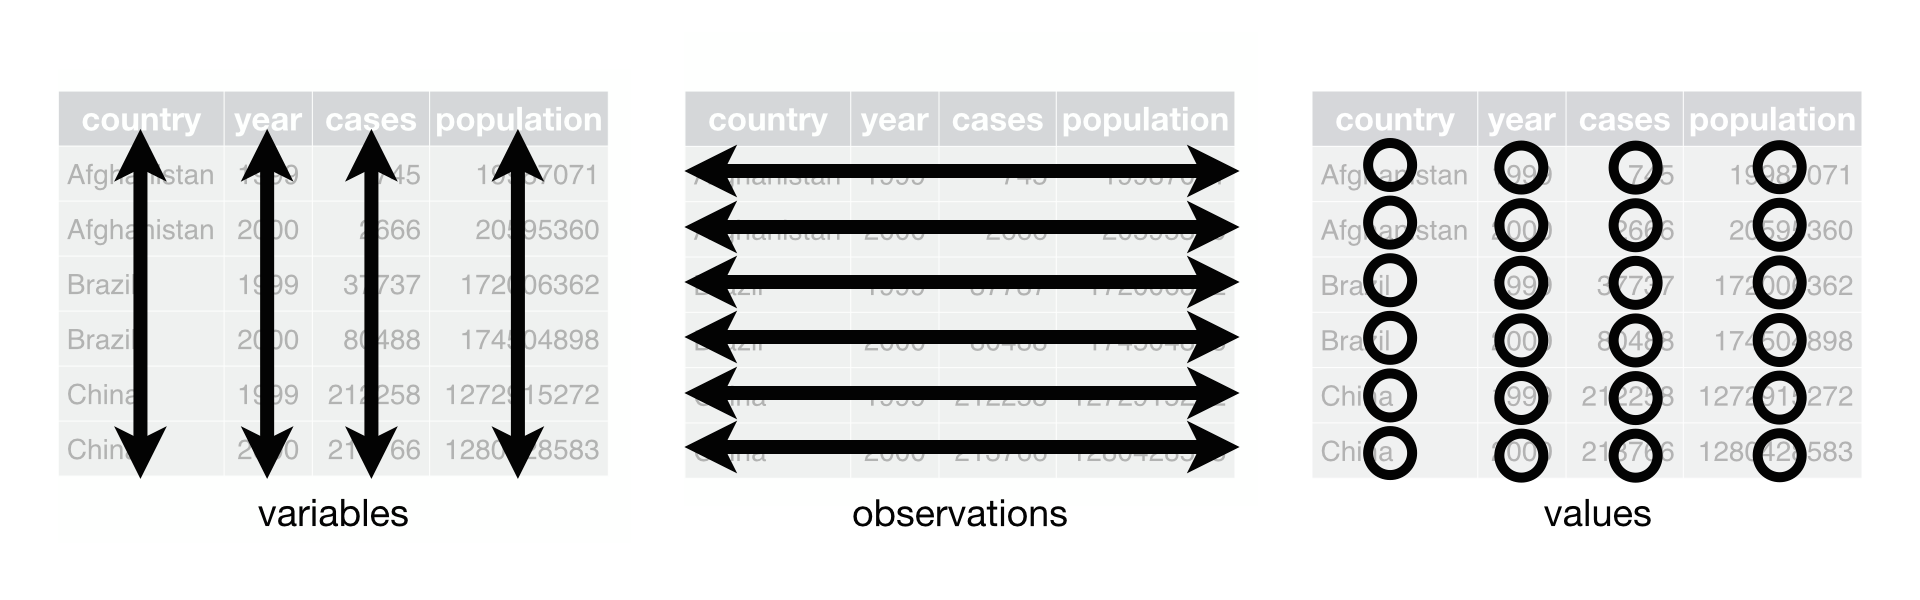
\includegraphics[width=6.4in,height=\textheight]{tidy-1.png}

}

\caption{Tidy data graphic from http://r4ds.had.co.nz/tidy-data.html}

\end{figure}%

For example, say the following table consists of stock prices:

\begingroup\fontsize{9}{11}\selectfont

\begin{longtable}[t]{llll}
\caption{\label{tab:unnamed-chunk-5}Stock Prices (Non-Tidy Format)}\\
\toprule
Date & Boeing Stock Price & Amazon Stock Price & Google Stock Price\\
\midrule
2009-01-01 & \$173.55 & \$174.90 & \$174.34\\
2009-01-02 & \$172.61 & \$171.42 & \$170.04\\
\bottomrule
\end{longtable}
\endgroup{}

Although the data are neatly organised in a spreadsheet-type format,
they are not in tidy format since there are three variables
corresponding to three unique pieces of information (Date, Stock Name,
and Stock Price), but there are not three columns. In tidy data format
each variable should be its own column, as shown below. Notice that both
tables present the same information, but in different formats.

\begingroup\fontsize{9}{11}\selectfont

\begin{longtable}[t]{lll}
\caption{\label{tab:unnamed-chunk-6}Stock Prices (Tidy Format)}\\
\toprule
Date & Stock Name & Stock Price\\
\midrule
2009-01-01 & Boeing & \$173.55\\
2009-01-02 & Boeing & \$172.61\\
2009-01-01 & Amazon & \$174.90\\
2009-01-02 & Amazon & \$171.42\\
2009-01-01 & Google & \$174.34\\
\addlinespace
2009-01-02 & Google & \$170.04\\
\bottomrule
\end{longtable}
\endgroup{}

However, consider the following table:

\begingroup\fontsize{9}{11}\selectfont

\begin{longtable}[t]{lll}
\caption{\label{tab:unnamed-chunk-7}Date, Boeing Price, Weather Data}\\
\toprule
Date & Boeing Price & Weather\\
\midrule
2009-01-01 & \$173.55 & Sunny\\
2009-01-02 & \$172.61 & Overcast\\
\bottomrule
\end{longtable}
\endgroup{}

In this case, even though the variable \textbf{Boeing Price} occurs
again, the data \emph{is} tidy since there are three variables
corresponding to three unique pieces of information (Date, Boeing stock
price, and the weather on that particular day).

The non-tidy data format in the original table is also known as
\href{https://en.wikipedia.org/wiki/Wide_and_narrow_data}{wide} format
whereas the tidy data format in the second table is also known as
\href{https://en.wikipedia.org/wiki/Wide_and_narrow_data\#Narrow}{long/narrow}
data format. In this course, we will work mostly with data sets that are
already in the tidy format.

\begin{tcolorbox}[enhanced jigsaw, title={Question}, bottomtitle=1mm, leftrule=.75mm, toprule=.15mm, opacityback=0, arc=.35mm, colbacktitle=quarto-callout-tip-color!10!white, bottomrule=.15mm, colback=white, coltitle=black, titlerule=0mm, toptitle=1mm, colframe=quarto-callout-tip-color-frame, opacitybacktitle=0.6, rightrule=.15mm, left=2mm, breakable]

Consider the following data frame of average number of servings of beer,
spirits, and wine consumption in three countries as reported in the
FiveThirtyEight article
\href{https://fivethirtyeight.com/features/dear-mona-followup-where-do-people-drink-the-most-beer-wine-and-spirits/}{Dear
Mona Followup: Where Do People Drink The Most Beer, Wine And Spirits?}

\begin{longtable}[]{@{}lrrr@{}}
\toprule\noalign{}
country & beer\_servings & spirit\_servings & wine\_servings \\
\midrule\noalign{}
\endhead
\bottomrule\noalign{}
\endlastfoot
Canada & 240 & 122 & 100 \\
South Korea & 140 & 16 & 9 \\
USA & 249 & 158 & 84 \\
\end{longtable}

This data frame is not in tidy format. What would it look like if it
were?

I need a hint

Think of these data as being in a wide format. What variables in this
data set could be placed in different columns?

See the solution

\begin{longtable}[]{@{}llr@{}}
\toprule\noalign{}
country & beverages type & number of servings \\
\midrule\noalign{}
\endhead
\bottomrule\noalign{}
\endlastfoot
Canada & beer\_servings & 240 \\
South Korea & beer\_servings & 140 \\
USA & beer\_servings & 249 \\
Canada & spirit\_servings & 122 \\
South Korea & spirit\_servings & 16 \\
USA & spirit\_servings & 158 \\
Canada & wine\_servings & 100 \\
South Korea & wine\_servings & 9 \\
USA & wine\_servings & 84 \\
\end{longtable}

\end{tcolorbox}

\section{\texorpdfstring{Converting to \textbf{tidy} data
format}{Converting to tidy data format}}\label{tidying}

In this section, we will see how to convert a data set that is not in
the \textbf{tidy} format
i.e.~\href{https://en.wikipedia.org/wiki/Wide_and_narrow_data}{wide}
format, to a data set that is in the \textbf{tidy} format
i.e.~\href{https://en.wikipedia.org/wiki/Wide_and_narrow_data\#Narrow}{long/narrow}
format.

First, let's download a \textbf{Comma Separated Values} (CSV) file of
ratings of the level of democracy in different countries spanning 1952
to 1992: \url{https://moderndive.com/data/dem_score.csv}. We use the
\texttt{read\_csv()} function from the \texttt{readr} package to read it
off the web:

\begin{Shaded}
\begin{Highlighting}[]
\NormalTok{dem\_score }\OtherTok{\textless{}{-}} \FunctionTok{read\_csv}\NormalTok{(}\StringTok{"https://moderndive.com/data/dem\_score.csv"}\NormalTok{)}
\end{Highlighting}
\end{Shaded}

\begin{tcolorbox}[enhanced jigsaw, title=\textcolor{quarto-callout-note-color}{\faInfo}\hspace{0.5em}{Note}, bottomtitle=1mm, leftrule=.75mm, toprule=.15mm, opacityback=0, arc=.35mm, colbacktitle=quarto-callout-note-color!10!white, bottomrule=.15mm, colback=white, coltitle=black, titlerule=0mm, toptitle=1mm, colframe=quarto-callout-note-color-frame, opacitybacktitle=0.6, rightrule=.15mm, left=2mm, breakable]

Please refer back to your \textbf{R programming} course for an overview
of how to import spreadsheets and \texttt{.csv} files into R.

\end{tcolorbox}

In this \texttt{dem\_score} data frame, the minimum value of -10
corresponds to a highly autocratic nation whereas a value of 10
corresponds to a highly democratic nation. Let's use the
\texttt{dem\_score} data frame but focus on only data corresponding to
the country of Guatemala.

\begin{Shaded}
\begin{Highlighting}[]
\NormalTok{guat\_dem }\OtherTok{\textless{}{-}}\NormalTok{  dplyr}\SpecialCharTok{::}\FunctionTok{filter}\NormalTok{(dem\_score,country }\SpecialCharTok{==} \StringTok{"Guatemala"}\NormalTok{)}
\NormalTok{guat\_dem}
\end{Highlighting}
\end{Shaded}

\begin{verbatim}
# A tibble: 1 x 10
  country   `1952` `1957` `1962` `1967` `1972` `1977` `1982` `1987` `1992`
  <chr>      <dbl>  <dbl>  <dbl>  <dbl>  <dbl>  <dbl>  <dbl>  <dbl>  <dbl>
1 Guatemala      2     -6     -5      3      1     -3     -7      3      3
\end{verbatim}

\begin{tcolorbox}[enhanced jigsaw, title=\textcolor{quarto-callout-note-color}{\faInfo}\hspace{0.5em}{Note}, bottomtitle=1mm, leftrule=.75mm, toprule=.15mm, opacityback=0, arc=.35mm, colbacktitle=quarto-callout-note-color!10!white, bottomrule=.15mm, colback=white, coltitle=black, titlerule=0mm, toptitle=1mm, colframe=quarto-callout-note-color-frame, opacitybacktitle=0.6, rightrule=.15mm, left=2mm, breakable]

Here we have used the \texttt{filter} function from \texttt{dplyr}
package to subset the data set. We will revisit this code for subsetting
data later in the session.

\end{tcolorbox}

In order for this data set to be on a \textbf{tidy} format, we need to
take the values of the current column names in \texttt{guat\_dem} (aside
from \texttt{country}) and convert them into a new variable that will
act as a key called \texttt{year}. Then, we'd like to take the numbers
on the inside of the table and turn them into a column that will act as
values called \texttt{democracy\_score}. Our resulting data frame will
have three columns: \texttt{country}, \texttt{year}, and
\texttt{democracy\_score}.

The \texttt{pivot\_longer} function in the \texttt{tidyr} package can
complete this task for us. The first argument to \texttt{pivot\_longer},
is the \texttt{data} argument where we specify which data frame we would
like to tidy. The next argument to \texttt{pivot\_longer} is
\texttt{cols} which specifies which columns we want to pivot into the
longer format.

\begin{tcolorbox}[enhanced jigsaw, title=\textcolor{quarto-callout-note-color}{\faInfo}\hspace{0.5em}{Note}, bottomtitle=1mm, leftrule=.75mm, toprule=.15mm, opacityback=0, arc=.35mm, colbacktitle=quarto-callout-note-color!10!white, bottomrule=.15mm, colback=white, coltitle=black, titlerule=0mm, toptitle=1mm, colframe=quarto-callout-note-color-frame, opacitybacktitle=0.6, rightrule=.15mm, left=2mm, breakable]

There are helper functions which help us declaring which variable (or
variables) we want to
pivot~\texttt{!},\texttt{start\_with},~\texttt{last\_col},~\texttt{everything},~\texttt{contains},
etc. E.g. \texttt{!country} will the tell the function that all the
variables except for \texttt{country} should be included in the pivoting
process.

\end{tcolorbox}

The next two arguments \texttt{names\_to} and \texttt{values\_to},
specify what we would like to call the new columns that convert our wide
data into tidy/long format.

\begin{Shaded}
\begin{Highlighting}[]
\NormalTok{guat\_dem\_long }\OtherTok{=} \FunctionTok{pivot\_longer}\NormalTok{(guat\_dem,}\AttributeTok{cols =} \SpecialCharTok{!}\NormalTok{country,}
                             \AttributeTok{names\_to =} \StringTok{"year"}\NormalTok{,}
                             \AttributeTok{values\_to =} \StringTok{"democracy\_score"}\NormalTok{)}
\FunctionTok{slice}\NormalTok{(guat\_dem\_long,}\DecValTok{1}\SpecialCharTok{:}\DecValTok{5}\NormalTok{)}
\end{Highlighting}
\end{Shaded}

\begin{verbatim}
# A tibble: 5 x 3
  country   year  democracy_score
  <chr>     <chr>           <dbl>
1 Guatemala 1952                2
2 Guatemala 1957               -6
3 Guatemala 1962               -5
4 Guatemala 1967                3
5 Guatemala 1972                1
\end{verbatim}

The inverse transformation of \texttt{pivot\_longer()} is of course,
\texttt{pivot\_wider()} and allows us to pivot from a long to a wide
format. As arguments we need to provide which column (or columns) to get
the name of the output column (\texttt{names\_from}), and which column
(or columns) to get the cell values from (\texttt{values\_from}). For
instance, if want the data from the previous example to go back to a
wide-format, we can use the following code:

\begin{Shaded}
\begin{Highlighting}[]
\NormalTok{guat\_dem\_wide }\OtherTok{=} \FunctionTok{pivot\_wider}\NormalTok{(guat\_dem\_long,}
                            \AttributeTok{names\_from =}\NormalTok{ year, }
                            \AttributeTok{values\_from =}\NormalTok{ democracy\_score)}
\NormalTok{guat\_dem\_wide}
\end{Highlighting}
\end{Shaded}

\begin{verbatim}
# A tibble: 1 x 10
  country   `1952` `1957` `1962` `1967` `1972` `1977` `1982` `1987` `1992`
  <chr>      <dbl>  <dbl>  <dbl>  <dbl>  <dbl>  <dbl>  <dbl>  <dbl>  <dbl>
1 Guatemala      2     -6     -5      3      1     -3     -7      3      3
\end{verbatim}

\begin{tcolorbox}[enhanced jigsaw, title={Task}, bottomtitle=1mm, leftrule=.75mm, toprule=.15mm, opacityback=0, arc=.35mm, colbacktitle=quarto-callout-warning-color!10!white, bottomrule=.15mm, colback=white, coltitle=black, titlerule=0mm, toptitle=1mm, colframe=quarto-callout-warning-color-frame, opacitybacktitle=0.6, rightrule=.15mm, left=2mm, breakable]

The information about drink consumption across countries is available on
the \texttt{drinks} data set in the \texttt{fivethirtyeight} library:

\begin{Shaded}
\begin{Highlighting}[]
\FunctionTok{library}\NormalTok{(fivethirtyeight)}
\NormalTok{drinks}
\end{Highlighting}
\end{Shaded}

\begin{longtable}[]{@{}
  >{\raggedright\arraybackslash}p{(\columnwidth - 8\tabcolsep) * \real{0.1412}}
  >{\raggedleft\arraybackslash}p{(\columnwidth - 8\tabcolsep) * \real{0.1647}}
  >{\raggedleft\arraybackslash}p{(\columnwidth - 8\tabcolsep) * \real{0.1882}}
  >{\raggedleft\arraybackslash}p{(\columnwidth - 8\tabcolsep) * \real{0.1647}}
  >{\raggedleft\arraybackslash}p{(\columnwidth - 8\tabcolsep) * \real{0.3412}}@{}}
\toprule\noalign{}
\begin{minipage}[b]{\linewidth}\raggedright
country
\end{minipage} & \begin{minipage}[b]{\linewidth}\raggedleft
beer\_servings
\end{minipage} & \begin{minipage}[b]{\linewidth}\raggedleft
spirit\_servings
\end{minipage} & \begin{minipage}[b]{\linewidth}\raggedleft
wine\_servings
\end{minipage} & \begin{minipage}[b]{\linewidth}\raggedleft
total\_litres\_of\_pure\_alcohol
\end{minipage} \\
\midrule\noalign{}
\endhead
\bottomrule\noalign{}
\endlastfoot
Afghanistan & 0 & 0 & 0 & 0.0 \\
Albania & 89 & 132 & 54 & 4.9 \\
Algeria & 25 & 0 & 14 & 0.7 \\
\end{longtable}

Convert this data frame to tidy data (long) format by pivoting the
variables related to the servings of beer, spirits and wine. Name the
new type of beverage column as \texttt{beverages\ type} and the servings
as \texttt{number\ of\ servings}.

Take hint

Your new data frame should contain 4 columns: \texttt{country},
\texttt{total\_litres\_of\_pure\_alcohol}, \texttt{beverages\ type} and
\texttt{number\ of\ servings}. You can use the \texttt{ends\_with()}
function to match variables according to a given pattern.

Click here to see the solution

\begin{Shaded}
\begin{Highlighting}[]
\CommentTok{\# There are multiples ways of doing this:}

\CommentTok{\# (1) We can explicitly declare which variable we don\textquotesingle{}t want to pivot}

\NormalTok{drinks }\SpecialCharTok{\%\textgreater{}\%}
  \FunctionTok{pivot\_longer}\NormalTok{(}\AttributeTok{cols =} \SpecialCharTok{!}\FunctionTok{c}\NormalTok{(country,total\_litres\_of\_pure\_alcohol),}
               \AttributeTok{names\_to =} \StringTok{"beverages type"}\NormalTok{,}
               \AttributeTok{values\_to =} \StringTok{"number of servings"}\NormalTok{)}

\CommentTok{\# (2) use a helper function to select the variables that end with the word "servings"}

\NormalTok{drinks }\SpecialCharTok{\%\textgreater{}\%}
  \FunctionTok{pivot\_longer}\NormalTok{(}\AttributeTok{cols =} \FunctionTok{ends\_with}\NormalTok{(}\StringTok{"servings"}\NormalTok{),}
               \AttributeTok{names\_to =} \StringTok{"beverages type"}\NormalTok{,}
               \AttributeTok{values\_to =} \StringTok{"number of servings"}\NormalTok{)}
\end{Highlighting}
\end{Shaded}

\end{tcolorbox}

\section{Reminder of ggplot}\label{reminder-of-ggplot}

Now that we have our data on a tidy format we can use \texttt{ggplot2}
to produce a plot showing how the democracy scores have changed over the
40 years from 1952 to 1992 for Guatemala. Lets have a reminder of how we
can do this using the ggplot.

First, we need to pass our data to the \texttt{ggplot()} function and
then add layers that can combines data, aesthetic mapping, a geom
(geometric object), a stat (statistical transformation), and a position
adjustment.

Let's start by laying out how we would map our aesthetics to variables
in the data frame:

\begin{itemize}
\tightlist
\item
  The \texttt{data} frame is \texttt{guat\_dem\_long} so we use
  \texttt{data\ =\ guat\_dem\_long}.
\item
  The mapping of the coordinates for the axes using
  \texttt{aes(x\ =\ year,\ y\ =\ democracy\_score)}, where
  \texttt{aes()} relates to the plots aesthetics. That is,

  \begin{itemize}
  \tightlist
  \item
    \texttt{year} maps to the \texttt{x} coordinate.
  \item
    \texttt{democracy\_score} maps to the \texttt{y} coordinate.
  \end{itemize}
\end{itemize}

Now we need to add an additional layer using the \texttt{+} command.
Lets include a points layer first:

\begin{Shaded}
\begin{Highlighting}[]
\FunctionTok{ggplot}\NormalTok{(}\AttributeTok{data =}\NormalTok{ guat\_dem\_long, }\AttributeTok{mapping =}\FunctionTok{aes}\NormalTok{(}\AttributeTok{x =}\NormalTok{ year, }\AttributeTok{y =}\NormalTok{ democracy\_score)) }\SpecialCharTok{+}
  \FunctionTok{geom\_point}\NormalTok{()}
\end{Highlighting}
\end{Shaded}

\begin{center}
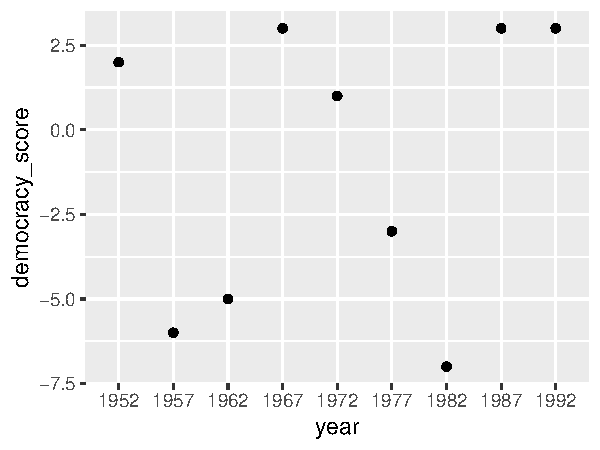
\includegraphics{notes_files/figure-pdf/Scatterplot Democracy vs. year-1.pdf}
\end{center}

When adding layers using \texttt{ggplot} it should be noted that:

\begin{itemize}
\tightlist
\item
  the \texttt{+} command should come at the end of lines, otherwise R
  will produce an error.
\item
  when adding additional layers it is a good idea to take a new line
  after each \texttt{+} command. This is so your code will be nice and
  clear with each layer given its own line of code. This is handy for
  code debugging.
\end{itemize}

Now we add a line connecting each point:

\begin{Shaded}
\begin{Highlighting}[]
\FunctionTok{ggplot}\NormalTok{(}\AttributeTok{data =}\NormalTok{ guat\_dem\_long, }\AttributeTok{mapping =}\FunctionTok{aes}\NormalTok{(}\AttributeTok{x =}\NormalTok{ year, }\AttributeTok{y =}\NormalTok{ democracy\_score)) }\SpecialCharTok{+}
  \FunctionTok{geom\_point}\NormalTok{()}\SpecialCharTok{+}
  \FunctionTok{geom\_line}\NormalTok{()}
\end{Highlighting}
\end{Shaded}

\begin{verbatim}
`geom_line()`: Each group consists of only one observation.
i Do you need to adjust the group aesthetic?
\end{verbatim}

\begin{center}
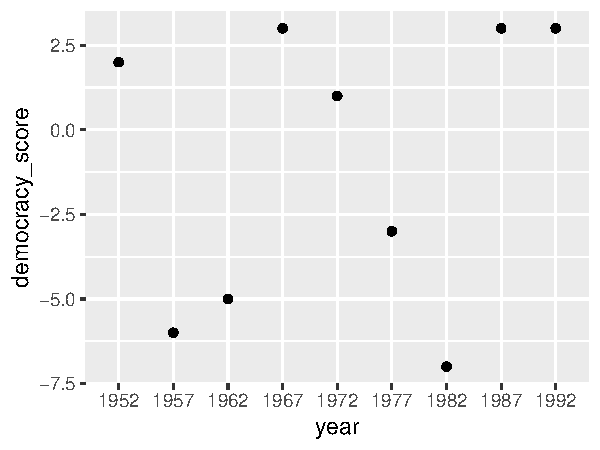
\includegraphics{notes_files/figure-pdf/unnamed-chunk-15-1.pdf}
\end{center}

\textbf{What happened?} Note that the \texttt{year} variable in
\texttt{guat\_dem\_long} is stored as a character vector since we had to
circumvent the naming rules in R by adding backticks around the
different year columns in \texttt{guat\_dem\_long}. This is leading to
\texttt{ggplot} not knowing exactly how to plot a line using a
categorical variable. We can fix this by using the
\texttt{parse\_number} function in the \texttt{readr} package:

\begin{Shaded}
\begin{Highlighting}[]
\FunctionTok{ggplot}\NormalTok{(}\AttributeTok{data =}\NormalTok{ guat\_dem\_long, }\AttributeTok{mapping =} \FunctionTok{aes}\NormalTok{(}\AttributeTok{x =} \FunctionTok{parse\_number}\NormalTok{(year), }\AttributeTok{y =}\NormalTok{ democracy\_score)) }\SpecialCharTok{+}
   \FunctionTok{geom\_point}\NormalTok{()}\SpecialCharTok{+}
   \FunctionTok{geom\_line}\NormalTok{()}
\end{Highlighting}
\end{Shaded}

\begin{center}
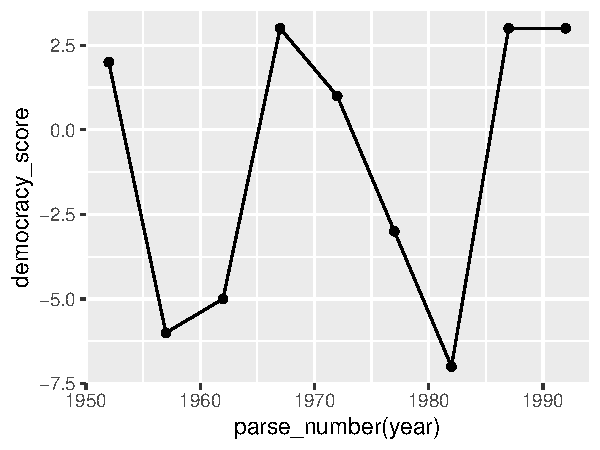
\includegraphics{notes_files/figure-pdf/unnamed-chunk-16-1.pdf}
\end{center}

We'll see later how we could use the \texttt{mutate} function to change
\texttt{year} to be a numeric variable during the tidying process
(alternatively we could have added the argument
\texttt{names\_transform\ =\ list(year\ =\ as.integer)} in the
\texttt{pivot\_longer()} function to declare the \texttt{year} column
values as an integers; see \texttt{?pivot\_longer} for more details).

As a final step we can change the axes labels and include a title on our
plot by adding another layer as follows:

\begin{Shaded}
\begin{Highlighting}[]
\FunctionTok{ggplot}\NormalTok{(}\AttributeTok{data =}\NormalTok{ guat\_dem\_long, }\AttributeTok{mapping =} \FunctionTok{aes}\NormalTok{(}\AttributeTok{x =} \FunctionTok{parse\_number}\NormalTok{(year), }\AttributeTok{y =}\NormalTok{ democracy\_score)) }\SpecialCharTok{+}
   \FunctionTok{geom\_point}\NormalTok{()}\SpecialCharTok{+}
   \FunctionTok{geom\_line}\NormalTok{()}\SpecialCharTok{+}
  \FunctionTok{labs}\NormalTok{(}\AttributeTok{x =} \StringTok{"year"}\NormalTok{, }\AttributeTok{y =} \StringTok{"Democracy score"}\NormalTok{,}
       \AttributeTok{title =} \StringTok{"Guatemala\textquotesingle{}s democracy score ratings from 1952 to 1992"}\NormalTok{)}
\end{Highlighting}
\end{Shaded}

\begin{center}
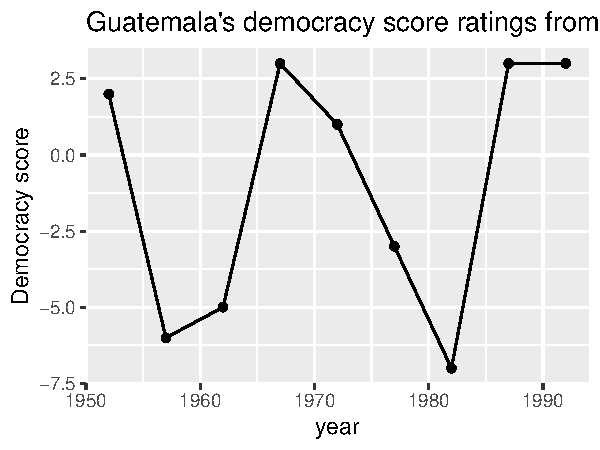
\includegraphics{notes_files/figure-pdf/unnamed-chunk-17-1.pdf}
\end{center}

\section{Data wrangling}\label{wrangling}

We are now able to import data and perform basic operations on the data
to get it into the \textbf{tidy} format. In this and subsequent sections
we will use tools from the \texttt{dplyr} package (included in
\texttt{tidyverse}) to perform data \textbf{wrangling} which includes
transforming, mapping and summarising variables.

\subsection{The pipe \%\textgreater\%}\label{piping}

Before we dig into data wrangling, let's first introduce the pipe
operator (\texttt{\%\textgreater{}\%}). Just as the \texttt{+} sign was
used to add layers to a plot created using \texttt{ggplot}, the pipe
operator allows us to chain together data wrangling functions. The pipe
operator can be read as \textbf{then}.

The piping syntax will be our major focus throughout the rest of this
course and you'll find that you'll quickly be addicted to the chaining
with some practice.

\subsection{Data wrangling verbs}\label{verbs}

The \texttt{d} in \texttt{dplyr} stands for data frames, so the
functions in \texttt{dplyr} are built for working with objects of the
data frame type. In your previous \textbf{R programming} course you have
already covered some of the most commonly used functions/verbs for
wrangling and summarising data (i.e.~\texttt{filter}, \texttt{summarise}
and \texttt{group\_by}). Thus, on this session we won't review these
deeply (for more details of how these verbs work please refer back to
your \textbf{R programming} course) but rather we will introduce new
verbs that you might not have seen before. Here is a description of some
of these verbs:

\begin{enumerate}
\def\labelenumi{\arabic{enumi}.}
\item
  \texttt{select}: Select variables in a data frame
\item
  \texttt{filter}: Pick rows based on conditions about their values
\item
  \texttt{summarize}: Compute summary measures known as ``summary
  statistics'' of variables
\item
  \texttt{group\_by}: Group rows of observations together
\item
  \texttt{mutate}: Create a new variable in the data frame by mutating
  existing ones
\item
  \texttt{join}: Join/merge two data frames by matching along a ``key''
  variable. There are many different \texttt{join} available. Here, we
  will focus on the \texttt{inner\_join} function.
\end{enumerate}

All of the verbs are used similarly where you: take a data frame, pipe
it using the \texttt{\%\textgreater{}\%} syntax into one of the verbs
above followed by other arguments specifying which criteria you would
like the verb to work with in parentheses.

\subsection{Select and rename columns}\label{select-and-rename-columns}

\begin{figure}[H]

{\centering 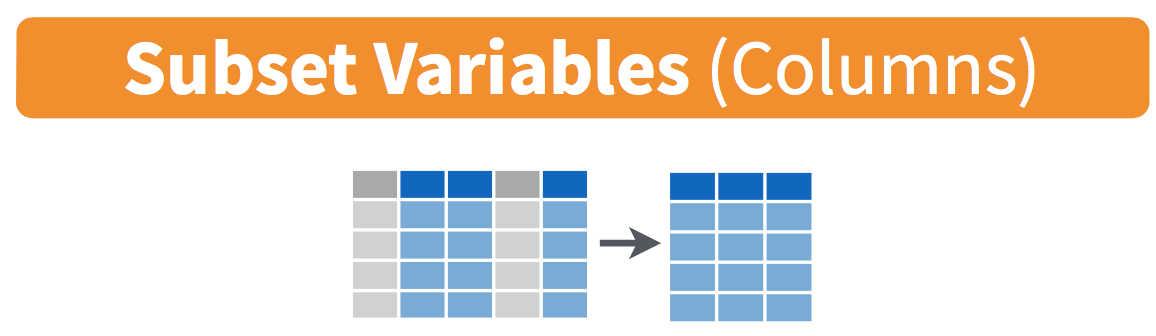
\includegraphics[width=3.85in,height=\textheight]{select.png}

}

\caption{Select diagram from Data Wrangling with dplyr and tidyr
cheatsheet.}

\end{figure}%

We've seen that the \texttt{flights} data frame in the
\texttt{nycflights13} package contains many different variables. The
\texttt{names} function gives a listing of all the columns in a data
frame; in our case you would run \texttt{names(flights)}. However, say
you only want to consider two of these variables, \texttt{carrier} and
\texttt{flight}. You can \texttt{select} these as follows:

\begin{Shaded}
\begin{Highlighting}[]
\NormalTok{flights }\SpecialCharTok{\%\textgreater{}\%}
  \FunctionTok{select}\NormalTok{(carrier, flight)}
\end{Highlighting}
\end{Shaded}

\begin{longtable}[]{@{}lr@{}}
\toprule\noalign{}
carrier & flight \\
\midrule\noalign{}
\endhead
\bottomrule\noalign{}
\endlastfoot
UA & 1545 \\
UA & 1714 \\
AA & 1141 \\
B6 & 725 \\
DL & 461 \\
\end{longtable}

The \texttt{select} function allows a subset of columns to be extracted,
making navigation data sets with a very large number of variables
easier.

Reversely, one can exclude specific columns via negative selection
(using -). For instance, in the \texttt{flights} data set, the
\texttt{year} variable isn't really a variable here in that it doesn't
vary (the \texttt{flights} data set actually comes from a larger data
set that covers many years). Thus, we may want to remove the
\texttt{year} variable from our data set since it won't be helpful for
analysis in this case. We can deselect \texttt{year} by using the
\texttt{-} sign:

\begin{Shaded}
\begin{Highlighting}[]
\NormalTok{flights\_no\_year }\OtherTok{\textless{}{-}}\NormalTok{ flights  }\SpecialCharTok{\%\textgreater{}\%} \FunctionTok{select}\NormalTok{(}\SpecialCharTok{{-}}\NormalTok{year)}
\end{Highlighting}
\end{Shaded}

The \texttt{select} function can also be used to reorder columns in
combination with the \texttt{everything} helper function. Let's suppose
we would like the \texttt{hour}, \texttt{minute}, and
\texttt{time\_hour} variables, which appear at the end of the
\texttt{flights} data set, to actually appear immediately after the
\texttt{day} variable:

\begin{Shaded}
\begin{Highlighting}[]
\NormalTok{flights\_reorder }\OtherTok{\textless{}{-}}\NormalTok{ flights }\SpecialCharTok{\%\textgreater{}\%}
  \FunctionTok{select}\NormalTok{(month}\SpecialCharTok{:}\NormalTok{day, hour}\SpecialCharTok{:}\NormalTok{time\_hour, }\FunctionTok{everything}\NormalTok{())}
\FunctionTok{names}\NormalTok{(flights\_reorder)}
\end{Highlighting}
\end{Shaded}

\begin{verbatim}
 [1] "month"          "day"            "hour"           "minute"        
 [5] "time_hour"      "year"           "dep_time"       "sched_dep_time"
 [9] "dep_delay"      "arr_time"       "sched_arr_time" "arr_delay"     
[13] "carrier"        "flight"         "tailnum"        "origin"        
[17] "dest"           "air_time"       "distance"      
\end{verbatim}

in this case \texttt{everything()} picks up all remaining variables.

\begin{tcolorbox}[enhanced jigsaw, title=\textcolor{quarto-callout-note-color}{\faInfo}\hspace{0.5em}{Note}, bottomtitle=1mm, leftrule=.75mm, toprule=.15mm, opacityback=0, arc=.35mm, colbacktitle=quarto-callout-note-color!10!white, bottomrule=.15mm, colback=white, coltitle=black, titlerule=0mm, toptitle=1mm, colframe=quarto-callout-note-color-frame, opacitybacktitle=0.6, rightrule=.15mm, left=2mm, breakable]

Alternatively we could use the \texttt{relocate()} verb to change column
positions, using the same syntax as \texttt{select()} to make it easy to
move blocks of columns at once. We will see an example of this in the
next section.

\end{tcolorbox}

Lastly, the helper functions \texttt{starts\_with}, \texttt{ends\_with},
and \texttt{contains} can be used to choose \textbf{variables / column
names} that match those conditions.

\begin{tcolorbox}[enhanced jigsaw, title={Task}, bottomtitle=1mm, leftrule=.75mm, toprule=.15mm, opacityback=0, arc=.35mm, colbacktitle=quarto-callout-warning-color!10!white, bottomrule=.15mm, colback=white, coltitle=black, titlerule=0mm, toptitle=1mm, colframe=quarto-callout-warning-color-frame, opacitybacktitle=0.6, rightrule=.15mm, left=2mm, breakable]

\begin{itemize}
\item
  Use \texttt{starts\_with} helper function to select the arrival time
  and arrival delay columns from the \texttt{flights} data frame.
\item
  Use \texttt{ends\_with} to select departure and arrival delay columns
  from the \texttt{flights} data frame.
\item
  Use \texttt{contains} to select columns to select departure times,
  schedule departure and departure delay columns from the
  \texttt{flights} data frame.
\end{itemize}

Take hint

In the \texttt{flights} data frame arrival time and arrival delay
columns all begin with the \texttt{arr} character, while departure and
arrival delay columns end with the \texttt{delay} character. Lastly,
departure times, schedule departure and departure delay columns all
contain the \texttt{dep} characters

Click here to see the solution

\begin{Shaded}
\begin{Highlighting}[]
\CommentTok{\# Select arrival time and arrival delay columns}
\NormalTok{flights }\SpecialCharTok{\%\textgreater{}\%}
  \FunctionTok{select}\NormalTok{(}\FunctionTok{starts\_with}\NormalTok{(}\StringTok{"arr"}\NormalTok{)) }\SpecialCharTok{\%\textgreater{}\%}
  \FunctionTok{slice}\NormalTok{(}\DecValTok{1}\SpecialCharTok{:}\DecValTok{3}\NormalTok{)}
\end{Highlighting}
\end{Shaded}

\begin{verbatim}
# A tibble: 3 x 2
  arr_time arr_delay
     <int>     <dbl>
1      830        11
2      850        20
3      923        33
\end{verbatim}

\begin{Shaded}
\begin{Highlighting}[]
\CommentTok{\# Select departure and arrival delay columns}
\NormalTok{flights }\SpecialCharTok{\%\textgreater{}\%}
  \FunctionTok{select}\NormalTok{(}\FunctionTok{ends\_with}\NormalTok{(}\StringTok{"delay"}\NormalTok{)) }\SpecialCharTok{\%\textgreater{}\%}
  \FunctionTok{slice}\NormalTok{(}\DecValTok{1}\SpecialCharTok{:}\DecValTok{3}\NormalTok{)}
\end{Highlighting}
\end{Shaded}

\begin{verbatim}
# A tibble: 3 x 2
  dep_delay arr_delay
      <dbl>     <dbl>
1         2        11
2         4        20
3         2        33
\end{verbatim}

\begin{Shaded}
\begin{Highlighting}[]
\CommentTok{\# Select departure times, schedule departure and departure delay columns}
\NormalTok{flights }\SpecialCharTok{\%\textgreater{}\%}
  \FunctionTok{select}\NormalTok{(}\FunctionTok{contains}\NormalTok{(}\StringTok{"dep"}\NormalTok{))}\SpecialCharTok{\%\textgreater{}\%}
  \FunctionTok{slice}\NormalTok{(}\DecValTok{1}\SpecialCharTok{:}\DecValTok{3}\NormalTok{)}
\end{Highlighting}
\end{Shaded}

\begin{verbatim}
# A tibble: 3 x 3
  dep_time sched_dep_time dep_delay
     <int>          <int>     <dbl>
1      517            515         2
2      533            529         4
3      542            540         2
\end{verbatim}

\end{tcolorbox}

Finally, if we want to rename a column while preserving the other
columns we can use the \texttt{rename} function. Suppose we wanted
\texttt{dep\_time} and \texttt{arr\_time} to be \texttt{departure\_time}
and \texttt{arrival\_time} instead in the \texttt{flights\_time} data
frame:

\begin{Shaded}
\begin{Highlighting}[]
\NormalTok{flights\_time }\OtherTok{\textless{}{-}}\NormalTok{ flights }\SpecialCharTok{\%\textgreater{}\%}
  \FunctionTok{select}\NormalTok{(}\FunctionTok{contains}\NormalTok{(}\StringTok{"time"}\NormalTok{)) }\SpecialCharTok{\%\textgreater{}\%}
  \FunctionTok{rename}\NormalTok{(}\AttributeTok{departure\_time =}\NormalTok{ dep\_time, }\AttributeTok{arrival\_time =}\NormalTok{ arr\_time)}
\FunctionTok{names}\NormalTok{(flights\_time)}
\end{Highlighting}
\end{Shaded}

\begin{verbatim}
[1] "departure_time" "sched_dep_time" "arrival_time"   "sched_arr_time"
[5] "air_time"       "time_hour"     
\end{verbatim}

Note that in this case we used a single \texttt{=} sign with
\texttt{rename}. e.g,. \texttt{departure\_time\ =\ dep\_time}. This is
because we are not testing for equality like we would using \texttt{==},
but instead we want to assign a new variable \texttt{departure\_time} to
have the same values as \texttt{dep\_time} and then delete the variable
\texttt{dep\_time}.

\subsection{Filter observations using filter}\label{filter}

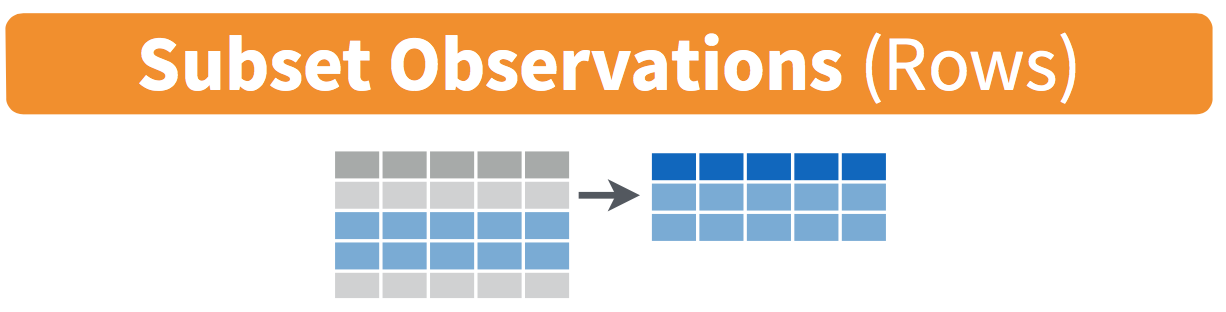
\includegraphics[width=4.09in,height=\textheight]{filter.png}

The \texttt{filter} function allows you to specify criteria about values
of a variable in your data set and then chooses only those rows that
match that criteria.

\begin{tcolorbox}[enhanced jigsaw, title=\textcolor{quarto-callout-important-color}{\faExclamation}\hspace{0.5em}{Important}, bottomtitle=1mm, leftrule=.75mm, toprule=.15mm, opacityback=0, arc=.35mm, colbacktitle=quarto-callout-important-color!10!white, bottomrule=.15mm, colback=white, coltitle=black, titlerule=0mm, toptitle=1mm, colframe=quarto-callout-important-color-frame, opacitybacktitle=0.6, rightrule=.15mm, left=2mm, breakable]

Recall that the base R has already a filter function defined. So make
sure to avoid any conflicts either by calling \texttt{dplyr::filter()}
every time you use the function (specially if you have loaded the
\texttt{conflicts} library) or alternatively run
the\texttt{conflict\_prefer()} function to let R know that it should use
\texttt{dplyr}'s \texttt{filter} function as default.

\begin{Shaded}
\begin{Highlighting}[]
\FunctionTok{conflict\_prefer}\NormalTok{(}\StringTok{"filter"}\NormalTok{, }\StringTok{"dplyr"}\NormalTok{)}
\end{Highlighting}
\end{Shaded}

\begin{verbatim}
[conflicted] Will prefer dplyr::filter over any other package.
\end{verbatim}

\end{tcolorbox}

Since you have already covered this in your \textbf{R programming
course}, let's begin straight away by focusing only at \emph{Alaska
Airlines} flights leaving from New York City in 2013. We can combine the
data wrangling output with ggplot plotting techniques. Run the following
code and look at the resulting scatterplot.

\begin{Shaded}
\begin{Highlighting}[]
\NormalTok{flights }\SpecialCharTok{\%\textgreater{}\%}
  \FunctionTok{filter}\NormalTok{(carrier }\SpecialCharTok{==}  \StringTok{"AS"}\NormalTok{) }\SpecialCharTok{\%\textgreater{}\%}
  \FunctionTok{ggplot}\NormalTok{(}\FunctionTok{aes}\NormalTok{(}\AttributeTok{x =}\NormalTok{ dep\_delay, }\AttributeTok{y =}\NormalTok{ arr\_delay)) }\SpecialCharTok{+}
  \FunctionTok{geom\_point}\NormalTok{()}\SpecialCharTok{+}
   \FunctionTok{labs}\NormalTok{(}\AttributeTok{x =} \StringTok{"Departure delay (minutes)"}\NormalTok{, }\AttributeTok{y =} \StringTok{"Arrival delay (minutes)"}\NormalTok{,}
       \AttributeTok{title =} \StringTok{"Alaska Airlines flights leaving NYC in 2013"}\NormalTok{)}
\end{Highlighting}
\end{Shaded}

\begin{center}
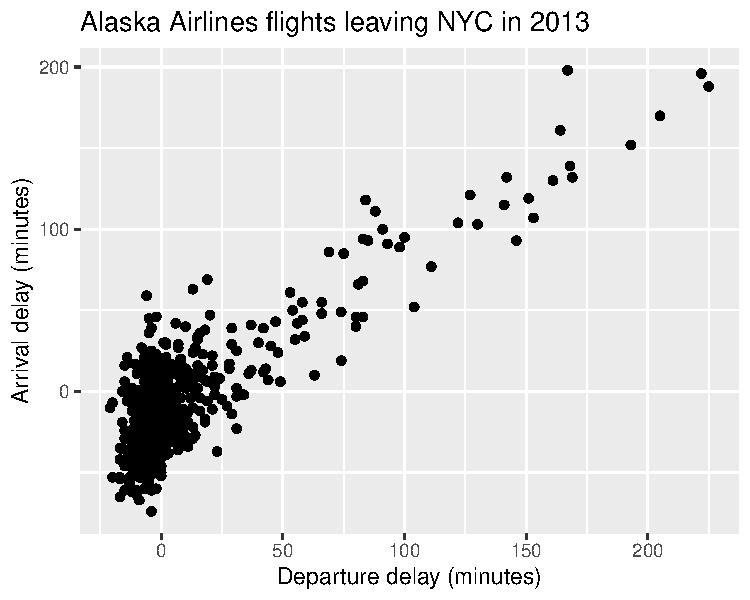
\includegraphics{notes_files/figure-pdf/Scatterplot Arrival vs Departue delays-1.pdf}
\end{center}

Here is an explanation of what we've just did:

\begin{itemize}
\tightlist
\item
  Take the data frame \texttt{flights} \textbf{then}
\item
  \texttt{filter} the data frame so that only those where the
  \texttt{carrier} equals \texttt{AS} are included. (recall that the
  double equals sign \texttt{==} tests equality, and not a single equals
  sign \texttt{=}).
\item
  pass the filtered data to the ggplot function and add a point layer
  and then modify axis labels.
\end{itemize}

You can combine multiple criteria together using operators that make
comparisons:

\begin{itemize}
\tightlist
\item
  \texttt{\textbar{}} corresponds to \textbf{or}
\item
  \texttt{\&} corresponds to \textbf{and}
\end{itemize}

We can often skip the use of \texttt{\&} and just separate our
conditions with a comma. You'll see this in the example below.

\begin{tcolorbox}[enhanced jigsaw, title=\textcolor{quarto-callout-note-color}{\faInfo}\hspace{0.5em}{Note}, bottomtitle=1mm, leftrule=.75mm, toprule=.15mm, opacityback=0, arc=.35mm, colbacktitle=quarto-callout-note-color!10!white, bottomrule=.15mm, colback=white, coltitle=black, titlerule=0mm, toptitle=1mm, colframe=quarto-callout-note-color-frame, opacitybacktitle=0.6, rightrule=.15mm, left=2mm, breakable]

In addition, you can use other mathematical checks (similar to
\texttt{==}):

\begin{itemize}
\item
  \texttt{\textgreater{}} corresponds to \textbf{greater than}
\item
  \texttt{\textless{}} corresponds to \textbf{less than}
\item
  \texttt{\textgreater{}=} corresponds to \textbf{greater than or equal
  to}
\item
  \texttt{\textless{}=} corresponds to \textbf{less than or equal to}
\item
  \texttt{!=} corresponds to \textbf{not equal to}
\end{itemize}

\end{tcolorbox}

To see many of these in action, let's select all flights that left JFK
airport heading to Burlington, Vermont (\texttt{BTV}) or Seattle,
Washington (\texttt{SEA}) in the months of October, November, or
December. Run the following:

\begin{Shaded}
\begin{Highlighting}[]
\NormalTok{btv\_sea\_flights\_fall }\OtherTok{\textless{}{-}}\NormalTok{ flights }\SpecialCharTok{\%\textgreater{}\%}
  \FunctionTok{filter}\NormalTok{(origin }\SpecialCharTok{==} \StringTok{"JFK"}\NormalTok{, (dest }\SpecialCharTok{==} \StringTok{"BTV"} \SpecialCharTok{|}\NormalTok{ dest }\SpecialCharTok{==} \StringTok{"SEA"}\NormalTok{), month }\SpecialCharTok{\textgreater{}=} \DecValTok{10}\NormalTok{) }\SpecialCharTok{\%\textgreater{}\%}
  \FunctionTok{relocate}\NormalTok{(dest,}\AttributeTok{.before =}\NormalTok{ dep\_time )}
\end{Highlighting}
\end{Shaded}

\begin{longtable}[]{@{}
  >{\raggedleft\arraybackslash}p{(\columnwidth - 36\tabcolsep) * \real{0.0298}}
  >{\raggedleft\arraybackslash}p{(\columnwidth - 36\tabcolsep) * \real{0.0357}}
  >{\raggedleft\arraybackslash}p{(\columnwidth - 36\tabcolsep) * \real{0.0238}}
  >{\raggedright\arraybackslash}p{(\columnwidth - 36\tabcolsep) * \real{0.0298}}
  >{\raggedleft\arraybackslash}p{(\columnwidth - 36\tabcolsep) * \real{0.0536}}
  >{\raggedleft\arraybackslash}p{(\columnwidth - 36\tabcolsep) * \real{0.0893}}
  >{\raggedleft\arraybackslash}p{(\columnwidth - 36\tabcolsep) * \real{0.0595}}
  >{\raggedleft\arraybackslash}p{(\columnwidth - 36\tabcolsep) * \real{0.0536}}
  >{\raggedleft\arraybackslash}p{(\columnwidth - 36\tabcolsep) * \real{0.0893}}
  >{\raggedleft\arraybackslash}p{(\columnwidth - 36\tabcolsep) * \real{0.0595}}
  >{\raggedright\arraybackslash}p{(\columnwidth - 36\tabcolsep) * \real{0.0476}}
  >{\raggedleft\arraybackslash}p{(\columnwidth - 36\tabcolsep) * \real{0.0417}}
  >{\raggedright\arraybackslash}p{(\columnwidth - 36\tabcolsep) * \real{0.0476}}
  >{\raggedright\arraybackslash}p{(\columnwidth - 36\tabcolsep) * \real{0.0417}}
  >{\raggedleft\arraybackslash}p{(\columnwidth - 36\tabcolsep) * \real{0.0536}}
  >{\raggedleft\arraybackslash}p{(\columnwidth - 36\tabcolsep) * \real{0.0536}}
  >{\raggedleft\arraybackslash}p{(\columnwidth - 36\tabcolsep) * \real{0.0298}}
  >{\raggedleft\arraybackslash}p{(\columnwidth - 36\tabcolsep) * \real{0.0417}}
  >{\raggedright\arraybackslash}p{(\columnwidth - 36\tabcolsep) * \real{0.1190}}@{}}
\toprule\noalign{}
\begin{minipage}[b]{\linewidth}\raggedleft
year
\end{minipage} & \begin{minipage}[b]{\linewidth}\raggedleft
month
\end{minipage} & \begin{minipage}[b]{\linewidth}\raggedleft
day
\end{minipage} & \begin{minipage}[b]{\linewidth}\raggedright
dest
\end{minipage} & \begin{minipage}[b]{\linewidth}\raggedleft
dep\_time
\end{minipage} & \begin{minipage}[b]{\linewidth}\raggedleft
sched\_dep\_time
\end{minipage} & \begin{minipage}[b]{\linewidth}\raggedleft
dep\_delay
\end{minipage} & \begin{minipage}[b]{\linewidth}\raggedleft
arr\_time
\end{minipage} & \begin{minipage}[b]{\linewidth}\raggedleft
sched\_arr\_time
\end{minipage} & \begin{minipage}[b]{\linewidth}\raggedleft
arr\_delay
\end{minipage} & \begin{minipage}[b]{\linewidth}\raggedright
carrier
\end{minipage} & \begin{minipage}[b]{\linewidth}\raggedleft
flight
\end{minipage} & \begin{minipage}[b]{\linewidth}\raggedright
tailnum
\end{minipage} & \begin{minipage}[b]{\linewidth}\raggedright
origin
\end{minipage} & \begin{minipage}[b]{\linewidth}\raggedleft
air\_time
\end{minipage} & \begin{minipage}[b]{\linewidth}\raggedleft
distance
\end{minipage} & \begin{minipage}[b]{\linewidth}\raggedleft
hour
\end{minipage} & \begin{minipage}[b]{\linewidth}\raggedleft
minute
\end{minipage} & \begin{minipage}[b]{\linewidth}\raggedright
time\_hour
\end{minipage} \\
\midrule\noalign{}
\endhead
\bottomrule\noalign{}
\endlastfoot
2013 & 10 & 1 & SEA & 729 & 735 & -6 & 1049 & 1040 & 9 & DL & 183 &
N721TW & JFK & 352 & 2422 & 7 & 35 & 2013-10-01 07:00:00 \\
2013 & 10 & 1 & SEA & 853 & 900 & -7 & 1217 & 1157 & 20 & B6 & 63 &
N807JB & JFK & 362 & 2422 & 9 & 0 & 2013-10-01 09:00:00 \\
2013 & 10 & 1 & BTV & 916 & 925 & -9 & 1016 & 1033 & -17 & B6 & 1634 &
N192JB & JFK & 48 & 266 & 9 & 25 & 2013-10-01 09:00:00 \\
\end{longtable}

\begin{tcolorbox}[enhanced jigsaw, title=\textcolor{quarto-callout-note-color}{\faInfo}\hspace{0.5em}{Note}, bottomtitle=1mm, leftrule=.75mm, toprule=.15mm, opacityback=0, arc=.35mm, colbacktitle=quarto-callout-note-color!10!white, bottomrule=.15mm, colback=white, coltitle=black, titlerule=0mm, toptitle=1mm, colframe=quarto-callout-note-color-frame, opacitybacktitle=0.6, rightrule=.15mm, left=2mm, breakable]

Even though colloquially speaking one might say ``all flights leaving
Burlington, Vermont \emph{and} Seattle, Washington,'' in terms of
computer logical operations, we really mean ``all flights leaving
Burlington, Vermont \emph{or} Seattle, Washington.'' For a given row in
the data, \texttt{dest} can be \texttt{BTV}, \texttt{SEA}, or something
else, but not \texttt{BTV} \textbf{and} \texttt{SEA} at the same time.
Also note that we have used the \texttt{relocate} function to change the
\texttt{dest} column position to just before the \texttt{dep\_time}. See
\texttt{?relocate} for further details.

\end{tcolorbox}

Another example uses \texttt{!} to pick rows that \emph{do not} match a
condition. The \texttt{!} can be read as \textbf{not}. Here, we are
selecting rows corresponding to flights that \textbf{did not} go to
Burlington, VT or Seattle, WA.

\begin{Shaded}
\begin{Highlighting}[]
\NormalTok{not\_BTV\_SEA }\OtherTok{\textless{}{-}}\NormalTok{ flights }\SpecialCharTok{\%\textgreater{}\%}
  \FunctionTok{filter}\NormalTok{(}\SpecialCharTok{!}\NormalTok{(dest }\SpecialCharTok{==} \StringTok{"BTV"} \SpecialCharTok{|}\NormalTok{ dest }\SpecialCharTok{==} \StringTok{"SEA"}\NormalTok{)) }\SpecialCharTok{\%\textgreater{}\%}
  \FunctionTok{relocate}\NormalTok{(dest,}\AttributeTok{.before =}\NormalTok{ dep\_time )}
\NormalTok{not\_BTV\_SEA }\SpecialCharTok{\%\textgreater{}\%}
  \FunctionTok{slice}\NormalTok{(}\DecValTok{1}\SpecialCharTok{:}\DecValTok{3}\NormalTok{)}
\end{Highlighting}
\end{Shaded}

\begin{verbatim}
# A tibble: 3 x 19
   year month   day dest  dep_time sched_dep_time dep_delay arr_time
  <int> <int> <int> <chr>    <int>          <int>     <dbl>    <int>
1  2013     1     1 IAH        517            515         2      830
2  2013     1     1 IAH        533            529         4      850
3  2013     1     1 MIA        542            540         2      923
# i 11 more variables: sched_arr_time <int>, arr_delay <dbl>, carrier <chr>,
#   flight <int>, tailnum <chr>, origin <chr>, air_time <dbl>, distance <dbl>,
#   hour <dbl>, minute <dbl>, time_hour <dttm>
\end{verbatim}

As a final note we point out that \texttt{filter} should often be the
first verb you'll apply to your data. This narrows down the data to just
the observations your are interested in.

\begin{tcolorbox}[enhanced jigsaw, title={Task}, bottomtitle=1mm, leftrule=.75mm, toprule=.15mm, opacityback=0, arc=.35mm, colbacktitle=quarto-callout-warning-color!10!white, bottomrule=.15mm, colback=white, coltitle=black, titlerule=0mm, toptitle=1mm, colframe=quarto-callout-warning-color-frame, opacitybacktitle=0.6, rightrule=.15mm, left=2mm, breakable]

What is another way of using the \textbf{not} operator \texttt{!} to
filter only the rows that are not going to Burlington, VT nor Seattle,
WA in the \texttt{flights} data frame?

Take a hint

Try using the \texttt{\%in\%} operator

Click here to see the solution

\begin{Shaded}
\begin{Highlighting}[]
\NormalTok{flights }\SpecialCharTok{\%\textgreater{}\%}
  \FunctionTok{filter}\NormalTok{( }\SpecialCharTok{!}\NormalTok{dest }\SpecialCharTok{\%in\%} \FunctionTok{c}\NormalTok{(}\StringTok{"BTV"}\NormalTok{,}\StringTok{"SEA"}\NormalTok{)) }\SpecialCharTok{\%\textgreater{}\%}
  \FunctionTok{head}\NormalTok{()}
\end{Highlighting}
\end{Shaded}

\begin{verbatim}
# A tibble: 6 x 19
   year month   day dep_time sched_dep_time dep_delay arr_time sched_arr_time
  <int> <int> <int>    <int>          <int>     <dbl>    <int>          <int>
1  2013     1     1      517            515         2      830            819
2  2013     1     1      533            529         4      850            830
3  2013     1     1      542            540         2      923            850
4  2013     1     1      544            545        -1     1004           1022
5  2013     1     1      554            600        -6      812            837
6  2013     1     1      554            558        -4      740            728
# i 11 more variables: arr_delay <dbl>, carrier <chr>, flight <int>,
#   tailnum <chr>, origin <chr>, dest <chr>, air_time <dbl>, distance <dbl>,
#   hour <dbl>, minute <dbl>, time_hour <dttm>
\end{verbatim}

\end{tcolorbox}

\subsection{Create new variables/change old variables using
mutate}\label{mutate}

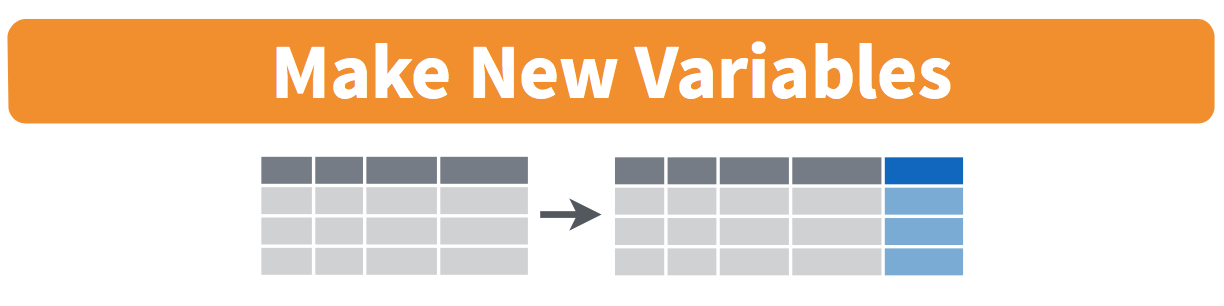
\includegraphics[width=4.08in,height=\textheight]{mutate.png}

When looking at the \texttt{flights} data set, there are some clear
additional variables that could be calculated based on the values of
variables already in the data set. Passengers are often frustrated when
their flights depart late, but change their mood a bit if pilots can
make up some time during the flight to get them to their destination
close to when they expected to land. This is commonly referred to as
``gain'' and we will create this variable using the \texttt{mutate}
function. Note that we will be overwriting the \texttt{flights} data
frame with one including the additional variable \texttt{gain} here, or
put differently, the \texttt{mutate} command outputs a new data frame
which then gets saved over the original \texttt{flights} data frame.

\begin{Shaded}
\begin{Highlighting}[]
\NormalTok{flights }\OtherTok{\textless{}{-}}\NormalTok{ flights }\SpecialCharTok{\%\textgreater{}\%}
  \FunctionTok{mutate}\NormalTok{(}\AttributeTok{gain =}\NormalTok{ dep\_delay }\SpecialCharTok{{-}}\NormalTok{ arr\_delay)}
\end{Highlighting}
\end{Shaded}

Let's take a look at \texttt{dep\_delay}, \texttt{arr\_delay}, and the
resulting \texttt{gain} variables in our new \texttt{flights} data
frame:

\begin{longtable}[]{@{}rrr@{}}
\toprule\noalign{}
dep\_delay & arr\_delay & gain \\
\midrule\noalign{}
\endhead
\bottomrule\noalign{}
\endlastfoot
2 & 11 & -9 \\
4 & 20 & -16 \\
2 & 33 & -31 \\
-1 & -18 & 17 \\
-6 & -25 & 19 \\
\end{longtable}

The flight in the first row departed 2 minutes late but arrived 11
minutes late, so its ``gained time in the air'' is actually a loss of 9
minutes, hence its \texttt{gain} is \texttt{-9}. Contrast this to the
flight in the fourth row which departed a minute early
(\texttt{dep\_delay} of \texttt{-1}) but arrived 18 minutes early
(\texttt{arr\_delay} of \texttt{-18}), so its ``gained time in the air''
is 17 minutes, hence its \texttt{gain} is \texttt{+17}.

\begin{tcolorbox}[enhanced jigsaw, title={Question}, bottomtitle=1mm, leftrule=.75mm, toprule=.15mm, opacityback=0, arc=.35mm, colbacktitle=quarto-callout-tip-color!10!white, bottomrule=.15mm, colback=white, coltitle=black, titlerule=0mm, toptitle=1mm, colframe=quarto-callout-tip-color-frame, opacitybacktitle=0.6, rightrule=.15mm, left=2mm, breakable]

Why did we overwrite \texttt{flights} instead of assigning the resulting
data frame to a new object, like \texttt{flights\_with\_gain}?

Answer

As a rough rule of thumb, as long as you are not losing information that
you might need later, it's acceptable practice to overwrite data frames.
However, if you overwrite existing variables and/or change the
observational units, recovering the original information might prove
difficult. In this case, it might make sense to create a new data
object.

\end{tcolorbox}

Let's look at visualize this \texttt{gain} variable in the form of a
histogram:

\begin{Shaded}
\begin{Highlighting}[]
\FunctionTok{ggplot}\NormalTok{(}\AttributeTok{data =}\NormalTok{ flights, }\AttributeTok{mapping =} \FunctionTok{aes}\NormalTok{(}\AttributeTok{x =}\NormalTok{ gain)) }\SpecialCharTok{+}
  \FunctionTok{geom\_histogram}\NormalTok{(}\AttributeTok{color =} \StringTok{"white"}\NormalTok{, }\AttributeTok{bins =} \DecValTok{20}\NormalTok{)}
\end{Highlighting}
\end{Shaded}

\begin{center}
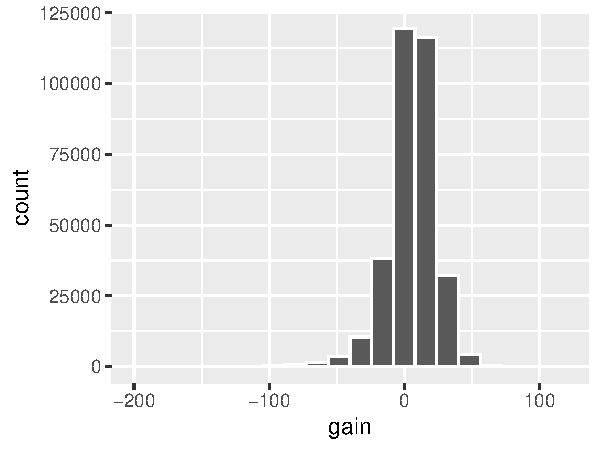
\includegraphics{notes_files/figure-pdf/Histogram of gained time-1.pdf}
\end{center}

We can also create multiple columns at once and even refer to columns
that were just created in a new column.

\begin{longtable}[]{@{}rrr@{}}
\toprule\noalign{}
gain & hours & gain\_per\_hour \\
\midrule\noalign{}
\endhead
\bottomrule\noalign{}
\endlastfoot
-9 & 3.783333 & -2.378855 \\
-16 & 3.783333 & -4.229075 \\
-31 & 2.666667 & -11.625000 \\
17 & 3.050000 & 5.573771 \\
19 & 1.933333 & 9.827586 \\
\end{longtable}

\begin{tcolorbox}[enhanced jigsaw, title={Question}, bottomtitle=1mm, leftrule=.75mm, toprule=.15mm, opacityback=0, arc=.35mm, colbacktitle=quarto-callout-tip-color!10!white, bottomrule=.15mm, colback=white, coltitle=black, titlerule=0mm, toptitle=1mm, colframe=quarto-callout-tip-color-frame, opacitybacktitle=0.6, rightrule=.15mm, left=2mm, breakable]

What do positive values of the \texttt{gain} variable in
\texttt{flights} correspond to?

\begin{itemize}
\tightlist
\item
  \begin{enumerate}
  \def\labelenumi{(\Alph{enumi})}
  \tightlist
  \item
    Departure delays are greater than arrivals delays\\
  \end{enumerate}
\item
  \begin{enumerate}
  \def\labelenumi{(\Alph{enumi})}
  \setcounter{enumi}{1}
  \tightlist
  \item
    Departure delays are lower than arrivals delays\\
  \end{enumerate}
\item
  \begin{enumerate}
  \def\labelenumi{(\Alph{enumi})}
  \setcounter{enumi}{2}
  \tightlist
  \item
    Departures and arrivals delays are the same
  \end{enumerate}
\end{itemize}

What about negative values?

\begin{itemize}
\tightlist
\item
  \begin{enumerate}
  \def\labelenumi{(\Alph{enumi})}
  \tightlist
  \item
    Departure delays are greater than arrivals delays\\
  \end{enumerate}
\item
  \begin{enumerate}
  \def\labelenumi{(\Alph{enumi})}
  \setcounter{enumi}{1}
  \tightlist
  \item
    Departure delays are lower than arrivals delays\\
  \end{enumerate}
\item
  \begin{enumerate}
  \def\labelenumi{(\Alph{enumi})}
  \setcounter{enumi}{2}
  \tightlist
  \item
    Departures and arrivals delays are the same
  \end{enumerate}
\end{itemize}

And what about a zero value?

\begin{itemize}
\tightlist
\item
  \begin{enumerate}
  \def\labelenumi{(\Alph{enumi})}
  \tightlist
  \item
    Departure delays are greater than arrivals delays\\
  \end{enumerate}
\item
  \begin{enumerate}
  \def\labelenumi{(\Alph{enumi})}
  \setcounter{enumi}{1}
  \tightlist
  \item
    Departuredelays are lower than arrivals delays\\
  \end{enumerate}
\item
  \begin{enumerate}
  \def\labelenumi{(\Alph{enumi})}
  \setcounter{enumi}{2}
  \tightlist
  \item
    Departures and arrivals delays are the same
  \end{enumerate}
\end{itemize}

\end{tcolorbox}

\begin{tcolorbox}[enhanced jigsaw, title={Question}, bottomtitle=1mm, leftrule=.75mm, toprule=.15mm, opacityback=0, arc=.35mm, colbacktitle=quarto-callout-tip-color!10!white, bottomrule=.15mm, colback=white, coltitle=black, titlerule=0mm, toptitle=1mm, colframe=quarto-callout-tip-color-frame, opacitybacktitle=0.6, rightrule=.15mm, left=2mm, breakable]

Could we create the \texttt{dep\_delay} and \texttt{arr\_delay} columns
by simply subtracting \texttt{dep\_time} from \texttt{sched\_dep\_time}
and similarly for arrivals? Try the code out and explain any differences
between the result and what actually appears in \texttt{flights}.

\begin{Shaded}
\begin{Highlighting}[]
\NormalTok{flights }\SpecialCharTok{\%\textgreater{}\%}
  \FunctionTok{mutate}\NormalTok{(}\AttributeTok{dep\_delay  =}\NormalTok{ sched\_dep\_time }\SpecialCharTok{{-}}\NormalTok{ dep\_time ,}
         \AttributeTok{arr\_delay  =}\NormalTok{ sched\_arr\_time  }\SpecialCharTok{{-}}\NormalTok{ arr\_time)}
\end{Highlighting}
\end{Shaded}

Take a hint

See the description of the variables \texttt{arr\_time},
\texttt{dep\_time}, \texttt{sched\_dep\_time} and
\texttt{sched\_arr\_time} in the flights data set \texttt{?flights}

Answer

The differences are due to departure and arrival times have a HHMM or
HMM format. E.g., if we compute the difference between a flight
scheduled to arrive by 923 and its actual arrival time at 850, the
result would be a difference of 73, while in reality there was only a 33
min difference if we consider the correct time format! We will see more
detials on how to work with time-date variables later on in this
session.

\end{tcolorbox}

\subsection{Summarise variables using summarize}\label{summarize}

The next common task is to be able to summarise data: take a large
number of values and summarise them with a single value. While this may
seem like a very abstract idea, something as simple as the sum, the
smallest value, and the largest values are all summaries of a large
number of values.

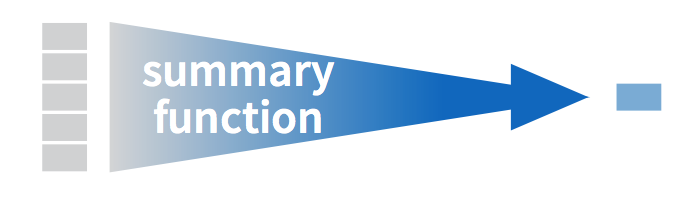
\includegraphics[width=2.29in,height=\textheight]{summary.png}

We can calculate the standard deviation and mean of the temperature
variable \texttt{temp} in the \texttt{weather} data frame of
\texttt{nycflights13} in one step using the \texttt{summarize} (or
equivalently using the UK spelling \texttt{summarise}) function in
\texttt{dplyr}. Before compute the mean it is important to notice that
there are some \textbf{missing values} in the data. Thus, by default any
time you try to summarise a number of values (using \texttt{mean()} and
\texttt{sd()} for example) that has one or more missing values, an
\texttt{NA} will be returned.

You can summarise all non-missing values by setting the \texttt{na.rm}
argument to TRUE (\texttt{rm} is short for remove). This will remove any
\texttt{NA} missing values and only return the summary value for all
non-missing values. So the code below computes the mean and standard
deviation of all non-missing values. Notice how the \texttt{na.rm=TRUE}
are set as arguments to the \texttt{mean} and \texttt{sd} functions, and
not to the \texttt{summarize} function.

\begin{Shaded}
\begin{Highlighting}[]
\NormalTok{summary\_temp }\OtherTok{\textless{}{-}}\NormalTok{ weather }\SpecialCharTok{\%\textgreater{}\%}
  \FunctionTok{summarize}\NormalTok{(}\AttributeTok{mean =} \FunctionTok{mean}\NormalTok{(temp, }\AttributeTok{na.rm =} \ConstantTok{TRUE}\NormalTok{), }\AttributeTok{std\_dev =} \FunctionTok{sd}\NormalTok{(temp, }\AttributeTok{na.rm =} \ConstantTok{TRUE}\NormalTok{))}
\NormalTok{summary\_temp}
\end{Highlighting}
\end{Shaded}

\begin{verbatim}
# A tibble: 1 x 2
   mean std_dev
  <dbl>   <dbl>
1  55.3    17.8
\end{verbatim}

\begin{tcolorbox}[enhanced jigsaw, title=\textcolor{quarto-callout-important-color}{\faExclamation}\hspace{0.5em}{Important}, bottomtitle=1mm, leftrule=.75mm, toprule=.15mm, opacityback=0, arc=.35mm, colbacktitle=quarto-callout-important-color!10!white, bottomrule=.15mm, colback=white, coltitle=black, titlerule=0mm, toptitle=1mm, colframe=quarto-callout-important-color-frame, opacitybacktitle=0.6, rightrule=.15mm, left=2mm, breakable]

It is \textbf{not} good practice to include \texttt{na.rm\ =\ TRUE} in
your summary commands by default; you should attempt to run code first
without this argument as this will alert you to the presence of missing
data. Only after you have identified where missing values occur and have
thought about the potential issues of these should you consider using
\texttt{na.rm\ =\ TRUE}.

\end{tcolorbox}

\begin{tcolorbox}[enhanced jigsaw, title={Question}, bottomtitle=1mm, leftrule=.75mm, toprule=.15mm, opacityback=0, arc=.35mm, colbacktitle=quarto-callout-tip-color!10!white, bottomrule=.15mm, colback=white, coltitle=black, titlerule=0mm, toptitle=1mm, colframe=quarto-callout-tip-color-frame, opacitybacktitle=0.6, rightrule=.15mm, left=2mm, breakable]

Say a doctor is studying the effect of smoking on lung cancer for a
large number of patients who have records measured at five year
intervals. She notices that a large number of patients have missing data
points because the patient has died, so she chooses to ignore these
patients in her analysis. What is wrong with this doctor's approach?

\begin{itemize}
\tightlist
\item
  \begin{enumerate}
  \def\labelenumi{(\Alph{enumi})}
  \tightlist
  \item
    Introduces a selection bias since patient who died due to lung
    cancer are excluded from the analysis, leading to an underestimation
    of the true impact of smoking on lung cancer risk\\
  \end{enumerate}
\item
  \begin{enumerate}
  \def\labelenumi{(\Alph{enumi})}
  \setcounter{enumi}{1}
  \tightlist
  \item
    There is no problem, smaller datasets with fewer missing values may
    require less computational resources, leading to faster processing
    times.\\
  \end{enumerate}
\item
  \begin{enumerate}
  \def\labelenumi{(\Alph{enumi})}
  \setcounter{enumi}{2}
  \tightlist
  \item
    Removing patients with missing data reduces the sample size. Hence,
    conclusions may not be as easily generalizable to the broader
    population, as the excluded patients may represent a different
    subset with unique characteristics.\\
  \end{enumerate}
\item
  \begin{enumerate}
  \def\labelenumi{(\Alph{enumi})}
  \setcounter{enumi}{3}
  \tightlist
  \item
    Removing missing values can result in a dataset with fewer errors
    and inconsistencies, which can lead to more accurate analyses.
  \end{enumerate}
\end{itemize}

\end{tcolorbox}

\subsection{Using grouping structures}\label{groupby}

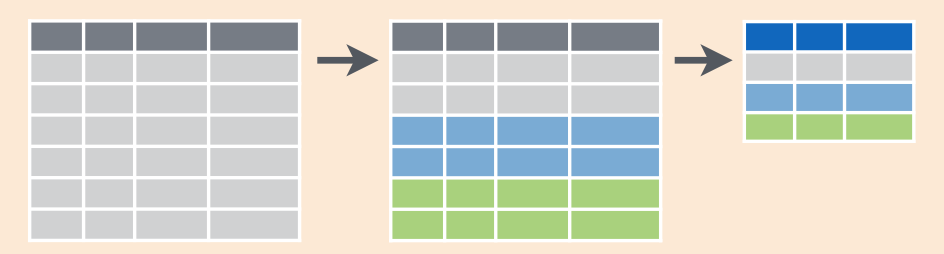
\includegraphics[width=3.15in,height=\textheight]{group_summary.png}

It is often more useful to summarise a variable based on the groupings
of another variable. Let's say we are interested in the mean and
standard deviation of temperatures but \emph{grouped by month}. Run the
following code:

\begin{Shaded}
\begin{Highlighting}[]
\NormalTok{summary\_monthly\_temp }\OtherTok{\textless{}{-}}\NormalTok{ weather }\SpecialCharTok{\%\textgreater{}\%}
  \FunctionTok{summarize}\NormalTok{(}\AttributeTok{mean =} \FunctionTok{mean}\NormalTok{(temp, }\AttributeTok{na.rm =} \ConstantTok{TRUE}\NormalTok{),}
            \AttributeTok{std\_dev =} \FunctionTok{sd}\NormalTok{(temp, }\AttributeTok{na.rm =} \ConstantTok{TRUE}\NormalTok{),}
            \AttributeTok{.by =}\NormalTok{ month)}
\end{Highlighting}
\end{Shaded}

This code is identical to the previous code that created
\texttt{summary\_temp}, with an extra \texttt{.by\ =\ month} added. This
kind per-operation grouping allow us to do the grouping within the
operation where the summarisation takes place without changing the
structure of the data .

\begin{tcolorbox}[enhanced jigsaw, title={Question}, bottomtitle=1mm, leftrule=.75mm, toprule=.15mm, opacityback=0, arc=.35mm, colbacktitle=quarto-callout-tip-color!10!white, bottomrule=.15mm, colback=white, coltitle=black, titlerule=0mm, toptitle=1mm, colframe=quarto-callout-tip-color-frame, opacitybacktitle=0.6, rightrule=.15mm, left=2mm, breakable]

The \texttt{drop\_na()} function can be used in the pipeline to remove
missing observations from a data set. Try running the following code to
compute the mean and standard deviation of the temperature in the
\texttt{weather} data set and comment on the output. Why is this
different from one one we had before?

\begin{Shaded}
\begin{Highlighting}[]
\NormalTok{summary\_monthly\_temp }\OtherTok{\textless{}{-}}\NormalTok{ weather }\SpecialCharTok{\%\textgreater{}\%}
  \FunctionTok{drop\_na}\NormalTok{() }\SpecialCharTok{\%\textgreater{}\%}
  \FunctionTok{summarize}\NormalTok{(}\AttributeTok{mean =} \FunctionTok{mean}\NormalTok{(temp),}
            \AttributeTok{std\_dev =} \FunctionTok{sd}\NormalTok{(temp),}
            \AttributeTok{.by =}\NormalTok{ month)}
\end{Highlighting}
\end{Shaded}

Answer

The \texttt{drop\_na()} function remove all missing observation from the
data set while specifying \texttt{na.rm\ =T} in each summarizing
function only removes the missing values for the specific variable to
which the function is applied.

\end{tcolorbox}

We now revisit the \texttt{n} counting summary function (see the
\textbf{R programming course} for more details). For example, suppose we
would like to get a sense for how many flights departed from each of the
three airports in New York City:

\begin{Shaded}
\begin{Highlighting}[]
\NormalTok{by\_origin }\OtherTok{\textless{}{-}}\NormalTok{ flights }\SpecialCharTok{\%\textgreater{}\%}
  \FunctionTok{summarize}\NormalTok{(}\AttributeTok{count =} \FunctionTok{n}\NormalTok{(),}
            \AttributeTok{.by =}\NormalTok{origin)}
\NormalTok{by\_origin}
\end{Highlighting}
\end{Shaded}

\begingroup\fontsize{9}{11}\selectfont

\begin{longtable*}[t]{lr}
\toprule
origin & count\\
\midrule
EWR & 120835\\
JFK & 111279\\
LGA & 104662\\
\bottomrule
\end{longtable*}
\endgroup{}

We see that Newark (\texttt{EWR}) had the most flights departing in 2013
followed by \texttt{JFK} and lastly by LaGuardia (\texttt{LGA}). Note,
there is a subtle but important difference between \texttt{sum} and
\texttt{n}. While \texttt{sum} simply adds up a large set of numbers,
the latter counts the number of times each of many different values
occur.

\begin{tcolorbox}[enhanced jigsaw, title={Task}, bottomtitle=1mm, leftrule=.75mm, toprule=.15mm, opacityback=0, arc=.35mm, colbacktitle=quarto-callout-warning-color!10!white, bottomrule=.15mm, colback=white, coltitle=black, titlerule=0mm, toptitle=1mm, colframe=quarto-callout-warning-color-frame, opacitybacktitle=0.6, rightrule=.15mm, left=2mm, breakable]

With the \texttt{weather} data set, write code to produce the mean and
standard deviation temperature for each day in 2013 for NYC.

Take a hint

See the documentation for \texttt{summarize()} (\texttt{?summarize})

Click here to see the solution

\begin{Shaded}
\begin{Highlighting}[]
\NormalTok{ weather }\SpecialCharTok{\%\textgreater{}\%}
  \FunctionTok{summarize}\NormalTok{(}\AttributeTok{mean =} \FunctionTok{mean}\NormalTok{(temp, }\AttributeTok{na.rm =} \ConstantTok{TRUE}\NormalTok{),}
            \AttributeTok{std\_dev =} \FunctionTok{sd}\NormalTok{(temp, }\AttributeTok{na.rm =} \ConstantTok{TRUE}\NormalTok{),}
            \AttributeTok{.by =}\NormalTok{ day)}
\end{Highlighting}
\end{Shaded}

\begin{verbatim}
# A tibble: 31 x 3
     day  mean std_dev
   <int> <dbl>   <dbl>
 1     1  57.6    17.4
 2     2  55.7    20.2
 3     3  53.8    18.9
 4     4  54.0    18.8
 5     5  55.6    16.2
 6     6  55.7    15.6
 7     7  55.6    17.4
 8     8  55.0    17.6
 9     9  56.6    17.4
10    10  56.9    17.8
# i 21 more rows
\end{verbatim}

\end{tcolorbox}

\subsection{Grouping by more than one
variable}\label{grouping-by-more-than-one-variable}

You are not limited to grouping by one variable. Say you wanted to know
the number of flights leaving each of the three New York City airports
\emph{for each month}, we can also group by a second variable
\texttt{month}:

\begin{Shaded}
\begin{Highlighting}[]
\NormalTok{by\_origin\_monthly }\OtherTok{\textless{}{-}}\NormalTok{ flights }\SpecialCharTok{\%\textgreater{}\%}
  \FunctionTok{summarize}\NormalTok{(}\AttributeTok{count =} \FunctionTok{n}\NormalTok{(),}
            \AttributeTok{.by =} \FunctionTok{c}\NormalTok{(origin, month))}
\NormalTok{by\_origin\_monthly}
\end{Highlighting}
\end{Shaded}

\begin{verbatim}
# A tibble: 36 x 3
   origin month count
   <chr>  <int> <int>
 1 EWR        1  9893
 2 LGA        1  7950
 3 JFK        1  9161
 4 EWR       10 10104
 5 JFK       10  9143
 6 LGA       10  9642
 7 JFK       11  8710
 8 EWR       11  9707
 9 LGA       11  8851
10 JFK       12  9146
# i 26 more rows
\end{verbatim}

We see there are 36 rows for \texttt{by\_origin\_monthly} because there
are 12 months times 3 airports (\texttt{EWR}, \texttt{JFK}, and
\texttt{LGA}). How can we visualize this information? Lets look now into
different techniques for manipulation and visualizing categorical data.

\section{Working with categorical
data}\label{working-with-categorical-data}

\subsection{Visualizing categorical
data}\label{visualizing-categorical-data}

Recall that barplots, or barcharts, are used to visualise the
distributions of categorical variables. This essentially provides us
with the frequencies of categories within a categorical variable. You
can use either the raw data (e.g.~the original \texttt{flights} data
set) or the summarised data set (e.g.~the \texttt{by\_origin\_monthly}
data set we just created) to create barplots in \texttt{ggplot.}

\section{Raw data and geom\_bar()}

Here we can use a data set with variable(s) representing the categories.
We can add a \texttt{geom\_bar()} layer to create a barplot layer by
counting the number of cases for each level of a categorical variable
and use the \texttt{fill=origin} option to assign a different color to
the counts based on the origin.

\begin{Shaded}
\begin{Highlighting}[]
\NormalTok{flights }\SpecialCharTok{\%\textgreater{}\%}
  \FunctionTok{ggplot}\NormalTok{(}\FunctionTok{aes}\NormalTok{(}\AttributeTok{x=}\FunctionTok{factor}\NormalTok{(month),}\AttributeTok{fill=}\NormalTok{origin))}\SpecialCharTok{+}
  \FunctionTok{geom\_bar}\NormalTok{()}\SpecialCharTok{+}
  \FunctionTok{scale\_x\_discrete}\NormalTok{(}\AttributeTok{labels =}\NormalTok{ month.abb) }\SpecialCharTok{+}
  \FunctionTok{labs}\NormalTok{(}\AttributeTok{x=} \StringTok{"Months"}\NormalTok{,}\AttributeTok{y=}\StringTok{"Number of flights"}\NormalTok{)}
\end{Highlighting}
\end{Shaded}

\begin{center}
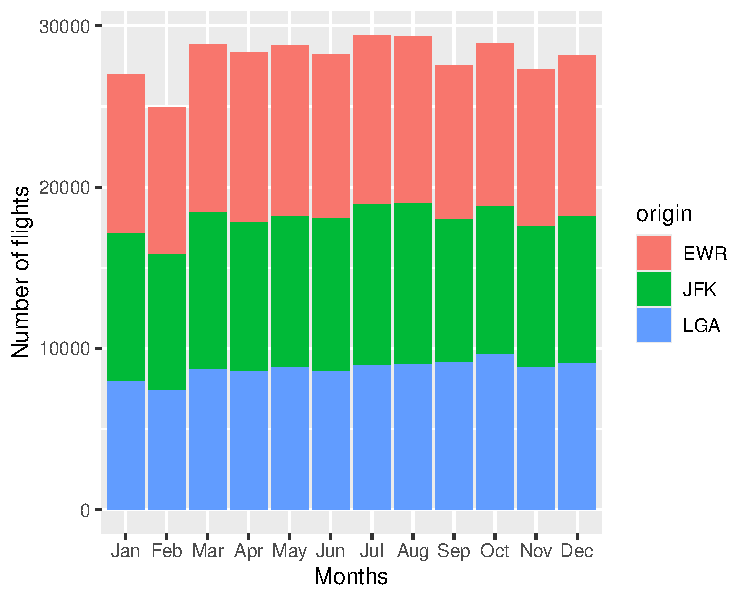
\includegraphics{notes_files/figure-pdf/Barplot for unaggregated count data-1.pdf}
\end{center}

Note that the month variable in our data set is an integer. Thus, we
convert this into a factor using the \texttt{factor()} function directly
in the aesthetic mapping. Then we provide appropriate labels for each
month (\texttt{labels\ =\ month.abb)} by adding one more
\texttt{scale\_x\_discrete}layer.

\section{Summarized data set and geom\_col()}

Here we can use a data set with variables representing the categories
and the counts of each category (e.g.~the \texttt{by\_origin\_monthly}
data set we just created). To produce the bar plot we add a
\texttt{geom\_col()} layer which expects a data set that already
contains the counts for each group. We use the \texttt{fill=origin}
option to assign a different color to the counts based on the origin.

\begin{Shaded}
\begin{Highlighting}[]
\NormalTok{by\_origin\_monthly }\SpecialCharTok{\%\textgreater{}\%}
\FunctionTok{ggplot}\NormalTok{(}\FunctionTok{aes}\NormalTok{(}\AttributeTok{x =} \FunctionTok{factor}\NormalTok{(month), }\AttributeTok{y =}\NormalTok{ count, }\AttributeTok{fill=}\NormalTok{ origin )) }\SpecialCharTok{+}
  \FunctionTok{geom\_col}\NormalTok{() }\SpecialCharTok{+}
  \FunctionTok{scale\_x\_discrete}\NormalTok{(}\AttributeTok{labels =}\NormalTok{ month.abb)}\SpecialCharTok{+}
    \FunctionTok{labs}\NormalTok{(}\AttributeTok{x=} \StringTok{"Months"}\NormalTok{,}\AttributeTok{y=}\StringTok{"Number of flights"}\NormalTok{)}
\end{Highlighting}
\end{Shaded}

\begin{center}
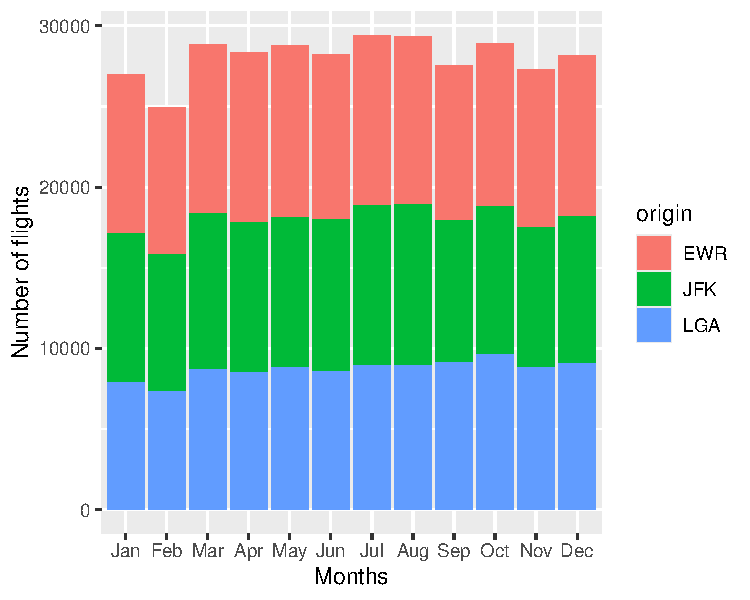
\includegraphics{notes_files/figure-pdf/Barplot for aggregated count data-1.pdf}
\end{center}

Note that the month variable in our data set is an integer. Thus, we
convert this into a factor using the \texttt{factor()} function directly
in the aesthetic mapping. Then we provide appropriate labels for each
month (\texttt{labels\ =\ month.abb)} by adding one more
\texttt{scale\_x\_discrete}layer.

This is what is referred to as a \emph{Stacked barplot} since the bars
for each \texttt{origin} are simply stacked on top of one another for
each of the carriers. This provides us with a visually nice barplot to
present the monthly number of flights by airport of origin. However,
there are also alternative barplots to the stacked barplot.

\begin{itemize}
\tightlist
\item
  One alternative to a stacked barplot is the \textbf{side-by-side} (or
  \textbf{dodged}) \textbf{barplot}, which, as suggested by its name,
  places the bars next to each other instead of on top of one another.
  This can be produced by including
  \texttt{position\ =\ \textquotesingle{}dodge\textquotesingle{}} within
  the \texttt{geom\_col} or \texttt{geom\_bar} layer.
\end{itemize}

\begin{tcolorbox}[enhanced jigsaw, title={Question}, bottomtitle=1mm, leftrule=.75mm, toprule=.15mm, opacityback=0, arc=.35mm, colbacktitle=quarto-callout-tip-color!10!white, bottomrule=.15mm, colback=white, coltitle=black, titlerule=0mm, toptitle=1mm, colframe=quarto-callout-tip-color-frame, opacitybacktitle=0.6, rightrule=.15mm, left=2mm, breakable]

How would you modify the code above to produced a \emph{dodged} barplot?

Answer

Depending on the structure of your data you could change the column/bar
layer to \texttt{geom\_col(position\ =\ "dodge")} or
\texttt{geom\_bar(position\ =\ "dodge")} respectively.

\end{tcolorbox}

\begin{itemize}
\tightlist
\item
  A second alternative is to use a \textbf{faceted barplot}. This can be
  produced by adding a \texttt{facet\_wrap()} layer to ggplot. E.g. try
  adding \texttt{facet\_wrap(\textasciitilde{}\ origin,\ ncol\ =\ 1)} to
  any of the previous barplots you have produced. The
  \texttt{facet\_wrap} function tells ggplot that we want to separate
  out barplots by \texttt{origin}, and hence we use
  \texttt{\textasciitilde{}\ origin}.
\end{itemize}

\begin{tcolorbox}[enhanced jigsaw, title={Task}, bottomtitle=1mm, leftrule=.75mm, toprule=.15mm, opacityback=0, arc=.35mm, colbacktitle=quarto-callout-warning-color!10!white, bottomrule=.15mm, colback=white, coltitle=black, titlerule=0mm, toptitle=1mm, colframe=quarto-callout-warning-color-frame, opacitybacktitle=0.6, rightrule=.15mm, left=2mm, breakable]

Boxplots are useful visualisations when comparing the distribution of a
numerical variable split across groups (or a categorical variable).
Taking the \texttt{weather} data set, use ggplot to create a boxplot
showing how the hourly temperature changes by month for each of the
three different Weather stations (\texttt{origin} variable). Use a
different color for each station.

Take a hint

To create boxplots using ggplot you can use the \texttt{geom\_boxplot}
function. If we want to look at boxplots of a variable separately for a
categorical variable then you need to declare that variable as a factor
using the \texttt{factor} function.

Click here to see the solution

\begin{Shaded}
\begin{Highlighting}[]
\FunctionTok{ggplot}\NormalTok{(}\AttributeTok{data =}\NormalTok{ weather, }\AttributeTok{mapping =} \FunctionTok{aes}\NormalTok{(}\AttributeTok{x =} \FunctionTok{factor}\NormalTok{(month), }\AttributeTok{y =}\NormalTok{ temp, }\AttributeTok{fill =}\NormalTok{ origin)) }\SpecialCharTok{+}
  \FunctionTok{geom\_boxplot}\NormalTok{() }\SpecialCharTok{+}
  \FunctionTok{facet\_wrap}\NormalTok{(}\SpecialCharTok{\textasciitilde{}}\NormalTok{origin)}\SpecialCharTok{+}
  \FunctionTok{labs}\NormalTok{(}\AttributeTok{x =} \StringTok{"Month"}\NormalTok{, }\AttributeTok{y =} \StringTok{"Temperature (Hourly)"}\NormalTok{,}
        \AttributeTok{title =} \StringTok{"Hourly temperatures from NYC in 2013 by month"}\NormalTok{)  }\SpecialCharTok{+}
   \FunctionTok{scale\_x\_discrete}\NormalTok{(}\AttributeTok{labels =}\NormalTok{ month.abb)}
\end{Highlighting}
\end{Shaded}

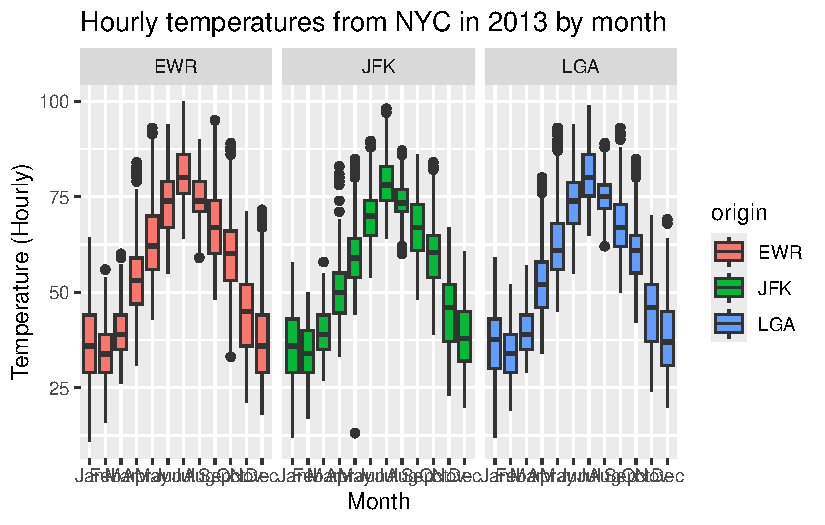
\includegraphics{notes_files/figure-pdf/unnamed-chunk-31-1.pdf}

\end{tcolorbox}

\begin{tcolorbox}[enhanced jigsaw, title={Task}, bottomtitle=1mm, leftrule=.75mm, toprule=.15mm, opacityback=0, arc=.35mm, colbacktitle=quarto-callout-warning-color!10!white, bottomrule=.15mm, colback=white, coltitle=black, titlerule=0mm, toptitle=1mm, colframe=quarto-callout-warning-color-frame, opacitybacktitle=0.6, rightrule=.15mm, left=2mm, breakable]

By using the \texttt{summarise()} function, how could we identify how
many flights left each of the three airports for each \texttt{carrier}?
Can you create a barplot showing these results?

Take a hint

You can count how many flights left each of the three airports by
summarising the data using the \texttt{n()} function while grouping by
the origin and carrier. Then, you can pass the resulting data frame to
\texttt{ggplot} using the pipeline command \texttt{\%\textgreater{}\%}
and use a \texttt{geom\_col} layer as in the previous example.

Click here to see the solution

\begin{Shaded}
\begin{Highlighting}[]
\NormalTok{flights }\SpecialCharTok{\%\textgreater{}\%}
  \FunctionTok{summarise}\NormalTok{(}\AttributeTok{count =} \FunctionTok{n}\NormalTok{(),}
            \AttributeTok{.by =} \FunctionTok{c}\NormalTok{(origin,carrier)) }\SpecialCharTok{\%\textgreater{}\%}
  \FunctionTok{ggplot}\NormalTok{(}\FunctionTok{aes}\NormalTok{(}\AttributeTok{x =}\NormalTok{ carrier, }\AttributeTok{y =}\NormalTok{ count, }\AttributeTok{fill =}\NormalTok{ origin)) }\SpecialCharTok{+} \FunctionTok{geom\_col}\NormalTok{()}
\end{Highlighting}
\end{Shaded}

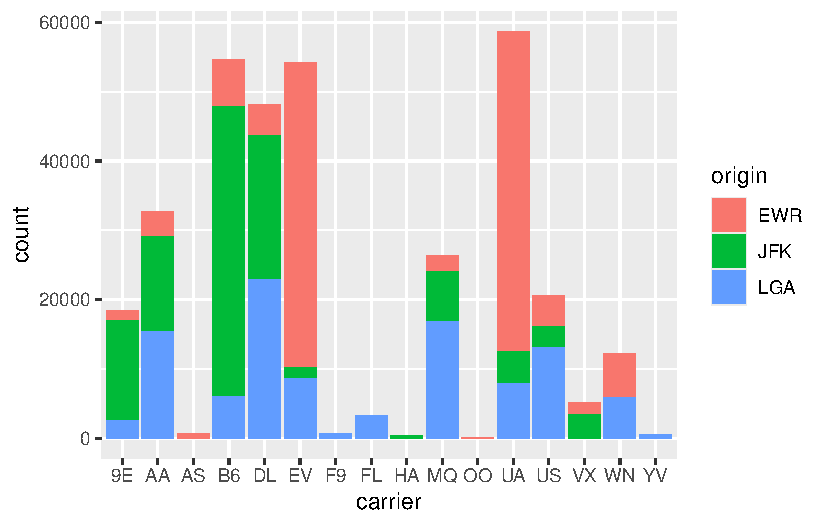
\includegraphics{notes_files/figure-pdf/unnamed-chunk-32-1.pdf}

\end{tcolorbox}

\subsection{\texorpdfstring{Vectorised if-else thru
\texttt{case\_when}}{Vectorised if-else thru case\_when}}\label{vectorised-if-else-thru-case_when}

In many situations, we may want to represent continuous variables as
discrete categories (e.g., grouping temperatures into ``cold,''
``warm,'' and ``hot'' ranges). The \texttt{case\_when} function provides
an efficient way to handle multiple if-else statements by vectorizing
them, allowing us to evaluate conditions and assign categories more
cleanly and concisely. In this session, we will use \texttt{case\_when}
to categorize weather conditions based on meteorological data from the
\texttt{weather} dataset. Let suppose that we want to categorize the
temperature variable into three categories:

\begin{itemize}
\item
  \textbf{low} for temperatures \(<39.9\)
\item
  \textbf{medium} for temperature values \(\geq 39.9\) and \(\leq 70\)
\item
  \textbf{high} for temperature values \(> 70\)
\end{itemize}

We can achieve this with the following code:

\begin{Shaded}
\begin{Highlighting}[]
\NormalTok{weather }\SpecialCharTok{\%\textgreater{}\%}
  \FunctionTok{mutate}\NormalTok{(}
    \AttributeTok{temp\_cat =} \FunctionTok{case\_when}\NormalTok{(}
      \FunctionTok{is.na}\NormalTok{(temp) }\SpecialCharTok{\textasciitilde{}} \ConstantTok{NA}\NormalTok{,}
\NormalTok{      temp }\SpecialCharTok{\textless{}} \FloatTok{39.9} \SpecialCharTok{\textasciitilde{}} \StringTok{"low"}\NormalTok{,}
      \FunctionTok{between}\NormalTok{(temp,}\FloatTok{39.9}\NormalTok{ ,}\DecValTok{70}\NormalTok{)}\SpecialCharTok{\textasciitilde{}} \StringTok{"medium"}\NormalTok{,}
      \AttributeTok{.default =} \StringTok{"large"}
\NormalTok{    )}
\NormalTok{  ) }\SpecialCharTok{\%\textgreater{}\%}
  \FunctionTok{relocate}\NormalTok{(temp,temp\_cat)}
\end{Highlighting}
\end{Shaded}

\begin{longtable}[]{@{}
  >{\raggedleft\arraybackslash}p{(\columnwidth - 30\tabcolsep) * \real{0.0476}}
  >{\raggedright\arraybackslash}p{(\columnwidth - 30\tabcolsep) * \real{0.0714}}
  >{\raggedright\arraybackslash}p{(\columnwidth - 30\tabcolsep) * \real{0.0556}}
  >{\raggedleft\arraybackslash}p{(\columnwidth - 30\tabcolsep) * \real{0.0397}}
  >{\raggedleft\arraybackslash}p{(\columnwidth - 30\tabcolsep) * \real{0.0476}}
  >{\raggedleft\arraybackslash}p{(\columnwidth - 30\tabcolsep) * \real{0.0317}}
  >{\raggedleft\arraybackslash}p{(\columnwidth - 30\tabcolsep) * \real{0.0397}}
  >{\raggedleft\arraybackslash}p{(\columnwidth - 30\tabcolsep) * \real{0.0476}}
  >{\raggedleft\arraybackslash}p{(\columnwidth - 30\tabcolsep) * \real{0.0476}}
  >{\raggedleft\arraybackslash}p{(\columnwidth - 30\tabcolsep) * \real{0.0714}}
  >{\raggedleft\arraybackslash}p{(\columnwidth - 30\tabcolsep) * \real{0.0873}}
  >{\raggedleft\arraybackslash}p{(\columnwidth - 30\tabcolsep) * \real{0.0794}}
  >{\raggedleft\arraybackslash}p{(\columnwidth - 30\tabcolsep) * \real{0.0556}}
  >{\raggedleft\arraybackslash}p{(\columnwidth - 30\tabcolsep) * \real{0.0714}}
  >{\raggedleft\arraybackslash}p{(\columnwidth - 30\tabcolsep) * \real{0.0476}}
  >{\raggedright\arraybackslash}p{(\columnwidth - 30\tabcolsep) * \real{0.1587}}@{}}
\toprule\noalign{}
\begin{minipage}[b]{\linewidth}\raggedleft
temp
\end{minipage} & \begin{minipage}[b]{\linewidth}\raggedright
temp\_cat
\end{minipage} & \begin{minipage}[b]{\linewidth}\raggedright
origin
\end{minipage} & \begin{minipage}[b]{\linewidth}\raggedleft
year
\end{minipage} & \begin{minipage}[b]{\linewidth}\raggedleft
month
\end{minipage} & \begin{minipage}[b]{\linewidth}\raggedleft
day
\end{minipage} & \begin{minipage}[b]{\linewidth}\raggedleft
hour
\end{minipage} & \begin{minipage}[b]{\linewidth}\raggedleft
dewp
\end{minipage} & \begin{minipage}[b]{\linewidth}\raggedleft
humid
\end{minipage} & \begin{minipage}[b]{\linewidth}\raggedleft
wind\_dir
\end{minipage} & \begin{minipage}[b]{\linewidth}\raggedleft
wind\_speed
\end{minipage} & \begin{minipage}[b]{\linewidth}\raggedleft
wind\_gust
\end{minipage} & \begin{minipage}[b]{\linewidth}\raggedleft
precip
\end{minipage} & \begin{minipage}[b]{\linewidth}\raggedleft
pressure
\end{minipage} & \begin{minipage}[b]{\linewidth}\raggedleft
visib
\end{minipage} & \begin{minipage}[b]{\linewidth}\raggedright
time\_hour
\end{minipage} \\
\midrule\noalign{}
\endhead
\bottomrule\noalign{}
\endlastfoot
39.02 & low & EWR & 2013 & 1 & 1 & 1 & 26.06 & 59.37 & 270 & 10.35702 &
NA & 0 & 1012.0 & 10 & 2013-01-01 01:00:00 \\
39.02 & low & EWR & 2013 & 1 & 1 & 2 & 26.96 & 61.63 & 250 & 8.05546 &
NA & 0 & 1012.3 & 10 & 2013-01-01 02:00:00 \\
39.02 & low & EWR & 2013 & 1 & 1 & 3 & 28.04 & 64.43 & 240 & 11.50780 &
NA & 0 & 1012.5 & 10 & 2013-01-01 03:00:00 \\
39.92 & medium & EWR & 2013 & 1 & 1 & 4 & 28.04 & 62.21 & 250 & 12.65858
& NA & 0 & 1012.2 & 10 & 2013-01-01 04:00:00 \\
39.02 & low & EWR & 2013 & 1 & 1 & 5 & 28.04 & 64.43 & 260 & 12.65858 &
NA & 0 & 1011.9 & 10 & 2013-01-01 05:00:00 \\
\end{longtable}

Here we use the \texttt{mutate} command to create new variable named
\texttt{temp\_cat}. The \texttt{case\_when} will then set to \texttt{NA}
those values in the original \texttt{temp} variable that are missing.
Then if the values of \texttt{temp} are \(< 30.9\) it will assign them
the label of \texttt{low}. If they lie between \(39.9\) and \(70\) it
will assign them the label of \texttt{medium} and finally set to
\texttt{large} any of the values that do not meet any of the
aforementioned conditions. We can also use the function
\texttt{relocate} to change the columns position so that the
\texttt{temp} and \texttt{temp\_cat} appears first on the data frame.

\begin{tcolorbox}[enhanced jigsaw, title={Task}, bottomtitle=1mm, leftrule=.75mm, toprule=.15mm, opacityback=0, arc=.35mm, colbacktitle=quarto-callout-warning-color!10!white, bottomrule=.15mm, colback=white, coltitle=black, titlerule=0mm, toptitle=1mm, colframe=quarto-callout-warning-color-frame, opacitybacktitle=0.6, rightrule=.15mm, left=2mm, breakable]

Create a new variable called \texttt{extreme\_weather} that takes the
value of \texttt{extreme} if the wind speed exceeds 64 mph and the
temperature is less than 40°F and \texttt{not\ extreme} otherwise. Then,
relocate this new variable along with the variables used to create it at
the first columns of the data frame, and sort them out based on
\texttt{wind\_speed}.

Take a hint

Use the conditional operators \texttt{\textbar{}} and \texttt{\&} to add
multiple conditions.

Click here to see the solution

\begin{Shaded}
\begin{Highlighting}[]
\NormalTok{weather }\SpecialCharTok{\%\textgreater{}\%}
  \FunctionTok{mutate}\NormalTok{(}
    \AttributeTok{extreme\_weather  =} \FunctionTok{case\_when}\NormalTok{(}
      \FunctionTok{is.na}\NormalTok{(temp)}\SpecialCharTok{|}\FunctionTok{is.na}\NormalTok{(wind\_speed) }\SpecialCharTok{\textasciitilde{}} \ConstantTok{NA}\NormalTok{,}
\NormalTok{      temp }\SpecialCharTok{\textless{}} \DecValTok{40} \SpecialCharTok{\&}\NormalTok{ wind\_speed  }\SpecialCharTok{\textgreater{}} \DecValTok{64}\SpecialCharTok{\textasciitilde{}} \StringTok{"extreme"}\NormalTok{,}
      \AttributeTok{.default =} \StringTok{"not extreme"}
\NormalTok{    )}
\NormalTok{  ) }\SpecialCharTok{\%\textgreater{}\%}
  \FunctionTok{relocate}\NormalTok{(extreme\_weather,temp,wind\_speed) }\SpecialCharTok{|\textgreater{}}
  \FunctionTok{arrange}\NormalTok{(}\FunctionTok{desc}\NormalTok{(wind\_speed))}
\end{Highlighting}
\end{Shaded}

\begin{verbatim}
# A tibble: 26,115 x 16
   extreme_weather  temp wind_speed origin  year month   day  hour  dewp humid
   <chr>           <dbl>      <dbl> <chr>  <int> <int> <int> <int> <dbl> <dbl>
 1 extreme          39.0     1048.  EWR     2013     2    12     3 27.0   61.6
 2 not extreme      57.2       42.6 EWR     2013     1    31     6 53.6   87.7
 3 not extreme      53.6       42.6 JFK     2013     1    31     4 53.1  100  
 4 not extreme      60.8       40.3 EWR     2013     1    31     4 59     93.8
 5 not extreme      59         40.3 LGA     2013     1    31     4 55.4   93.7
 6 not extreme      46.0       39.1 EWR     2013     1    31     8 30.0   53.3
 7 not extreme      41         38.0 JFK     2013     3     6    14 28.9   61.9
 8 not extreme      53.1       36.8 JFK     2013     1    31     3 52.0  100  
 9 not extreme      51.8       36.8 JFK     2013     1    31     7 46.4   81.7
10 not extreme      28.0       36.8 JFK     2013    11    24    10 -0.04  29.2
# i 26,105 more rows
# i 6 more variables: wind_dir <dbl>, wind_gust <dbl>, precip <dbl>,
#   pressure <dbl>, visib <dbl>, time_hour <dttm>
\end{verbatim}

\end{tcolorbox}

\section{Joining data frames}\label{joins}

Another common task is joining (merging) two different data sets. For
example, in the \texttt{flights} data, the variable \texttt{carrier}
lists the carrier code for the different flights. While \texttt{UA} and
\texttt{AA} might be somewhat easy to guess for some (United and
American Airlines), what are VX, HA, and B6? This information is
provided in a separate data frame \texttt{airlines}.

\begin{Shaded}
\begin{Highlighting}[]
\NormalTok{airlines}
\end{Highlighting}
\end{Shaded}

\begin{longtable}[]{@{}ll@{}}
\toprule\noalign{}
carrier & name \\
\midrule\noalign{}
\endhead
\bottomrule\noalign{}
\endlastfoot
9E & Endeavor Air Inc. \\
AA & American Airlines Inc. \\
AS & Alaska Airlines Inc. \\
B6 & JetBlue Airways \\
DL & Delta Air Lines Inc. \\
\end{longtable}

We see that in \texttt{airports}, \texttt{carrier} is the carrier code
while \texttt{name} is the full name of the airline. Using this table,
we can map the carrier in the \texttt{flights} data set to its
corresponding full name stored in the \texttt{airlines} data. However,
will we have to continually look up the carrier's name for each flight
in the \texttt{airlines} data set?

No! Instead of having to do this manually, we can have R automatically
do the ``looking up'' for us.

Note that the values in the variable \texttt{carrier} in
\texttt{flights} match the values in the variable \texttt{carrier} in
\texttt{airlines}. In this case, we can use the variable
\texttt{carrier} as a \emph{key variable} to join/merge/match the two
data frames by. Key variables are almost always identification variables
that uniquely identify the observational units. This ensures that rows
in both data frames are appropriately matched during the join. This
diagram helps us understand how the different data sets are linked by
various key variables:

\begin{figure}[H]

{\centering 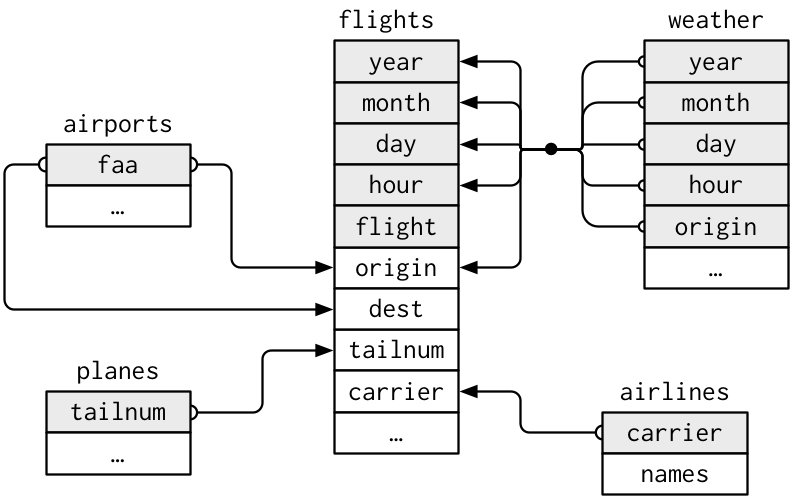
\includegraphics[width=2.64in,height=\textheight]{relational-nycflights.png}

}

\caption{Data relationships in nycflights13 from R for Data Science,
Hadley and Garrett (2016).}

\end{figure}%

\subsection{Joining by ``key''
variables}\label{joining-by-key-variables}

In both \texttt{flights} and \texttt{airlines}, the key variable we want
to join/merge/match the two data frames with has the same name in both
data sets: \texttt{carriers}. We make use of the \texttt{inner\_join}
function to join by the variable \texttt{carrier}.

\begin{Shaded}
\begin{Highlighting}[]
\NormalTok{flights\_joined }\OtherTok{\textless{}{-}}\NormalTok{ flights }\SpecialCharTok{\%\textgreater{}\%}
  \FunctionTok{inner\_join}\NormalTok{(airlines,}
             \AttributeTok{by =} \FunctionTok{join\_by}\NormalTok{(carrier))}
\end{Highlighting}
\end{Shaded}

If we compare the \texttt{flights} and the \texttt{flights\_joined} we
just created, we will observe that these are identical except that
\texttt{flights\_joined} has an additional variable \texttt{name} whose
values were drawn from \texttt{airlines}.

A visual representation of the \texttt{inner\_join} is given below:

\begin{figure}[H]

{\centering 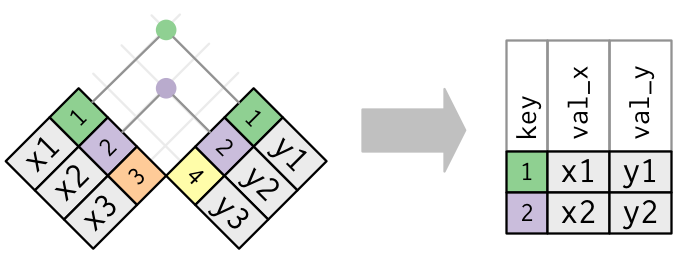
\includegraphics[width=2.25in,height=\textheight]{join-inner.png}

}

\caption{Diagram of inner join from R for Data Science.}

\end{figure}%

There are more complex joins available, but the \texttt{inner\_join}
will solve nearly all of the problems you will face here.

\subsection{Joining by ``key'' variables with different
names}\label{joining-by-key-variables-with-different-names}

Say instead, you are interested in all the destinations of flights from
NYC in 2013 and ask yourself:

\begin{itemize}
\tightlist
\item
  ``What cities are these airports in?''
\item
  ``Is \texttt{ORD} Orlando?''
\item
  ``Where is \texttt{FLL}?''
\end{itemize}

The \texttt{airports} data frame contains airport codes:

\begin{Shaded}
\begin{Highlighting}[]
\NormalTok{airports}
\end{Highlighting}
\end{Shaded}

\begin{longtable}[]{@{}
  >{\raggedright\arraybackslash}p{(\columnwidth - 14\tabcolsep) * \real{0.0488}}
  >{\raggedright\arraybackslash}p{(\columnwidth - 14\tabcolsep) * \real{0.3659}}
  >{\raggedleft\arraybackslash}p{(\columnwidth - 14\tabcolsep) * \real{0.1098}}
  >{\raggedleft\arraybackslash}p{(\columnwidth - 14\tabcolsep) * \real{0.1220}}
  >{\raggedleft\arraybackslash}p{(\columnwidth - 14\tabcolsep) * \real{0.0610}}
  >{\raggedleft\arraybackslash}p{(\columnwidth - 14\tabcolsep) * \real{0.0366}}
  >{\raggedright\arraybackslash}p{(\columnwidth - 14\tabcolsep) * \real{0.0488}}
  >{\raggedright\arraybackslash}p{(\columnwidth - 14\tabcolsep) * \real{0.2073}}@{}}
\toprule\noalign{}
\begin{minipage}[b]{\linewidth}\raggedright
faa
\end{minipage} & \begin{minipage}[b]{\linewidth}\raggedright
name
\end{minipage} & \begin{minipage}[b]{\linewidth}\raggedleft
lat
\end{minipage} & \begin{minipage}[b]{\linewidth}\raggedleft
lon
\end{minipage} & \begin{minipage}[b]{\linewidth}\raggedleft
alt
\end{minipage} & \begin{minipage}[b]{\linewidth}\raggedleft
tz
\end{minipage} & \begin{minipage}[b]{\linewidth}\raggedright
dst
\end{minipage} & \begin{minipage}[b]{\linewidth}\raggedright
tzone
\end{minipage} \\
\midrule\noalign{}
\endhead
\bottomrule\noalign{}
\endlastfoot
04G & Lansdowne Airport & 41.13047 & -80.61958 & 1044 & -5 & A &
America/New\_York \\
06A & Moton Field Municipal Airport & 32.46057 & -85.68003 & 264 & -6 &
A & America/Chicago \\
06C & Schaumburg Regional & 41.98934 & -88.10124 & 801 & -6 & A &
America/Chicago \\
06N & Randall Airport & 41.43191 & -74.39156 & 523 & -5 & A &
America/New\_York \\
09J & Jekyll Island Airport & 31.07447 & -81.42778 & 11 & -5 & A &
America/New\_York \\
\end{longtable}

However, looking at both the \texttt{airports} and \texttt{flights} and
the visual representation of the relations between the data frames in
the figure above, we see that in:

\begin{itemize}
\tightlist
\item
  \texttt{airports} the airport code is in the variable \texttt{faa}
\item
  \texttt{flights} the airport code is in the variable \texttt{origin}
\end{itemize}

So to join these two data sets, our \texttt{inner\_join} operation
involves a logical operator \texttt{==} argument that accounts for the
different names.

\begin{Shaded}
\begin{Highlighting}[]
\NormalTok{flights }\SpecialCharTok{\%\textgreater{}\%}
  \FunctionTok{inner\_join}\NormalTok{(airports,}
             \AttributeTok{by =} \FunctionTok{join\_by}\NormalTok{(dest }\SpecialCharTok{==}\NormalTok{ faa))}
\end{Highlighting}
\end{Shaded}

We can read the code out loud as:

``\emph{Take the flights data frame and inner join it to the airports
data frame by the entries where the variable} \texttt{dest} \emph{is
equal to} \texttt{faa}''

Let's construct the sequence of commands that computes the number of
flights from NYC to each destination, but also includes information
about each destination airport:

\begin{Shaded}
\begin{Highlighting}[]
\NormalTok{named\_dests }\OtherTok{\textless{}{-}}\NormalTok{ flights }\SpecialCharTok{\%\textgreater{}\%}
  \FunctionTok{summarize}\NormalTok{(}\AttributeTok{num\_flights =} \FunctionTok{n}\NormalTok{(),}
            \AttributeTok{.by =}\NormalTok{ dest)  }\SpecialCharTok{\%\textgreater{}\%}
  \FunctionTok{arrange}\NormalTok{(}\FunctionTok{desc}\NormalTok{(num\_flights))  }\SpecialCharTok{\%\textgreater{}\%}
  \FunctionTok{inner\_join}\NormalTok{(airports, }\AttributeTok{by =} \FunctionTok{join\_by}\NormalTok{(dest }\SpecialCharTok{==}\NormalTok{ faa)) }\SpecialCharTok{\%\textgreater{}\%}
  \FunctionTok{rename}\NormalTok{(}\AttributeTok{airport\_name =}\NormalTok{ name)}
\NormalTok{named\_dests}
\end{Highlighting}
\end{Shaded}

\begin{verbatim}
# A tibble: 5 x 9
  dest  num_flights airport_name              lat    lon   alt    tz dst   tzone
  <chr>       <int> <chr>                   <dbl>  <dbl> <dbl> <dbl> <chr> <chr>
1 ORD         17283 Chicago Ohare Intl       42.0  -87.9   668    -6 A     Amer~
2 ATL         17215 Hartsfield Jackson Atl~  33.6  -84.4  1026    -5 A     Amer~
3 LAX         16174 Los Angeles Intl         33.9 -118.    126    -8 A     Amer~
4 BOS         15508 General Edward Lawrenc~  42.4  -71.0    19    -5 A     Amer~
5 MCO         14082 Orlando Intl             28.4  -81.3    96    -5 A     Amer~
\end{verbatim}

In case you didn't know, \texttt{ORD} is the airport code of Chicago
O'Hare airport and \texttt{FLL} is the main airport in Fort Lauderdale,
Florida, which we can now see in our \texttt{named\_dests} data frame.

\subsection{Joining by multiple ``key''
variables}\label{joining-by-multiple-key-variables}

Say instead we are in a situation where we need to join by multiple
variables. For example, in the first figure in this section we see that
in order to join the \texttt{flights} and \texttt{weather} data frames,
we need more than one key variable: \texttt{year}, \texttt{month},
\texttt{day}, \texttt{hour}, and \texttt{origin}. This is because the
combination of these 5 variables act to uniquely identify each
observational unit in the \texttt{weather} data frame: hourly weather
recordings at each of the 3 NYC airports.

We achieve this by specifying a vector of key variables to join by.

\begin{Shaded}
\begin{Highlighting}[]
\NormalTok{flights\_weather\_joined }\OtherTok{\textless{}{-}}\NormalTok{ flights  }\SpecialCharTok{\%\textgreater{}\%}
  \FunctionTok{inner\_join}\NormalTok{(weather,}
             \AttributeTok{by =} \FunctionTok{join\_by}\NormalTok{(year,month,day,hour,origin))}

\NormalTok{flights\_weather\_joined}
\end{Highlighting}
\end{Shaded}

\begin{verbatim}
# A tibble: 335,220 x 32
    year month   day dep_time sched_dep_time dep_delay arr_time sched_arr_time
   <int> <int> <int>    <int>          <int>     <dbl>    <int>          <int>
 1  2013     1     1      517            515         2      830            819
 2  2013     1     1      533            529         4      850            830
 3  2013     1     1      542            540         2      923            850
 4  2013     1     1      544            545        -1     1004           1022
 5  2013     1     1      554            600        -6      812            837
 6  2013     1     1      554            558        -4      740            728
 7  2013     1     1      555            600        -5      913            854
 8  2013     1     1      557            600        -3      709            723
 9  2013     1     1      557            600        -3      838            846
10  2013     1     1      558            600        -2      753            745
# i 335,210 more rows
# i 24 more variables: arr_delay <dbl>, carrier <chr>, flight <int>,
#   tailnum <chr>, origin <chr>, dest <chr>, air_time <dbl>, distance <dbl>,
#   hour <dbl>, minute <dbl>, time_hour.x <dttm>, gain <dbl>, hours <dbl>,
#   gain_per_hour <dbl>, temp <dbl>, dewp <dbl>, humid <dbl>, wind_dir <dbl>,
#   wind_speed <dbl>, wind_gust <dbl>, precip <dbl>, pressure <dbl>,
#   visib <dbl>, time_hour.y <dttm>
\end{verbatim}

\begin{tcolorbox}[enhanced jigsaw, title={Question}, bottomtitle=1mm, leftrule=.75mm, toprule=.15mm, opacityback=0, arc=.35mm, colbacktitle=quarto-callout-tip-color!10!white, bottomrule=.15mm, colback=white, coltitle=black, titlerule=0mm, toptitle=1mm, colframe=quarto-callout-tip-color-frame, opacitybacktitle=0.6, rightrule=.15mm, left=2mm, breakable]

Looking at the first figure in this section, when joining
\texttt{flights} and \texttt{weather} (or, in other words, matching the
hourly weather values with each flight), why do we need to join by all
of \texttt{year}, \texttt{month}, \texttt{day}, \texttt{hour}, and
\texttt{origin}, and not just \texttt{hour}?

Answer

\texttt{year},\texttt{month},\texttt{day},\texttt{hour},\texttt{origin}
are the key variables that allow us to uniquely identify the
observational units.

\end{tcolorbox}

\begin{tcolorbox}[enhanced jigsaw, title={Task}, bottomtitle=1mm, leftrule=.75mm, toprule=.15mm, opacityback=0, arc=.35mm, colbacktitle=quarto-callout-warning-color!10!white, bottomrule=.15mm, colback=white, coltitle=black, titlerule=0mm, toptitle=1mm, colframe=quarto-callout-warning-color-frame, opacitybacktitle=0.6, rightrule=.15mm, left=2mm, breakable]

Create a new data frame that shows the top 5 airports with the largest
average arrival delays from NYC in 2013.

Take a hint

Compute the mean arrival delay from each destination. You can then join
the resulting data set with the \texttt{airports} data which contains
the airports names and search for the top 5 entries.

Click here to see the solution

\begin{Shaded}
\begin{Highlighting}[]
\NormalTok{  flights }\SpecialCharTok{\%\textgreater{}\%}
  \FunctionTok{summarize}\NormalTok{(}\AttributeTok{mean\_arr\_delay =} \FunctionTok{mean}\NormalTok{(arr\_delay,}\AttributeTok{na.rm=}\NormalTok{T),}
            \AttributeTok{.by =}\NormalTok{ dest)  }\SpecialCharTok{\%\textgreater{}\%}
  \FunctionTok{inner\_join}\NormalTok{(airports, }\AttributeTok{by =} \FunctionTok{join\_by}\NormalTok{(dest }\SpecialCharTok{==}\NormalTok{ faa)) }\SpecialCharTok{\%\textgreater{}\%}
  \FunctionTok{rename}\NormalTok{(}\AttributeTok{airport\_name =}\NormalTok{ name) }\SpecialCharTok{|\textgreater{}}
    \FunctionTok{slice\_max}\NormalTok{(mean\_arr\_delay,}\AttributeTok{n=}\DecValTok{5}\NormalTok{)}
\end{Highlighting}
\end{Shaded}

\end{tcolorbox}

\section*{The end?}\label{the-end}
\addcontentsline{toc}{section}{The end?}

Congratulations! You have reached the end of today's session. But wait,
there's still more! To further enhance your skills in Data analysis,
check out the additional material provided on handling date-time data.
This will help you learn how to manage and manipulate date-time
variables within the framework of tidy data, enabling you to perform
more precise and effective analyses.



\end{document}
